% Refer back to them as e.g. equation~(\ref{eq:quadratic}).

% Figures are referred to as e.g. Fig.~\ref{fig:example_figure}, and tables as
% e.g. Table~\ref{tab:example_table}.

 % The \cite command functions as follows:
 %   \citet{key} ==>>                Jones et al. (1990)
 %   \citet*{key} ==>>               Jones, Baker, and Smith (1990)
 %   \citep{key} ==>>                (Jones et al., 1990)
 %   \citep*{key} ==>>               (Jones, Baker, and Smith, 1990)
 %   \citep[chap. 2]{key} ==>>       (Jones et al., 1990, chap. 2)
 %   \citep[e.g.][]{key} ==>>        (e.g. Jones et al., 1990)
 %   \citep[e.g.][p. 32]{key} ==>>   (e.g. Jones et al., p. 32)
 %   \citeauthor{key} ==>>           Jones et al.
 %   \citeauthor*{key} ==>>          Jones, Baker, and Smith
 %   \citeyear{key} ==>>             1990
 %---------------------------------------------------------------------
%%%%%%%%%%%%%%%%%%%%%%%%%%%%%%%%%%%%%%%%%%%%%%%%%%
% Basic setup. Most papers should leave these options alone.
% \documentclass[a4paper,fleqn,usenatbib,draft]{mnras}
\documentclass[fleqn,usenatbib]{mnras}

\usepackage{natbib}
\usepackage{soul}

% MNRAS is set in Times font. If you don't have this installed (most LaTeX
% installations will be fine) or prefer the old Computer Modern fonts, comment
% out the following line

% Depending on your LaTeX fonts installation, you might get better results with one of these:
% \usepackage{mathptmx}
% \usepackage{txfonts}

% Use vector fonts, so it zooms properly in on-screen viewing software
% Don't change these lines unless you know what you are doing
\usepackage[T1]{fontenc}
\usepackage{ae,aecompl}


%%%%% AUTHORS - PLACE YOUR OWN PACKAGES HERE %%%%%
%\usepackage{todonotes}
\usepackage{outlines}
\usepackage{color}

% Only include extra packages if you really need them. Common packages are:
\usepackage{graphicx}	% Including figure files
\usepackage{amsmath}	% Advanced maths commands
\usepackage{amssymb}	% Extra maths symbols
\usepackage{bm}	        % bold font in math
\usepackage{newtxtext,newtxmath}
\usepackage{hyperref}

\usepackage{ulem}
%%%%%%%%%%%%%%%%%%%%%%%%%%%%%%%%%%%%%%%%%%%%%%%%%%

%%%%% AUTHORS - PLACE YOUR OWN COMMANDS HERE %%%%%

% \hypersetup{draft}
% annotation for math!
% \newcommand\allbold[1]{{\boldmath\textbf{#1}}}
% \newcommand\allbold[1]{ {\color{red} {\boldmath\textbf{#1}} } }
\newcommand\allbold[1]{ {\color{red} {#1} } }
\usepackage{natbib}

\def\xihm{\xi_{\mathrm{hm}}}
\def\ximm{\xi_{\mathrm{mm}}}
\def\mrm{\mathrm}

\defcitealias{Zu2021}{Z21}
\defcitealias{Zibetti2005}{Z05}

\newcommand{\rsoi}{R_{\mathrm{SOI}}}
\newcommand{\sigbi}{\Sigma_*^{\texttt{B+I}}}
\newcommand{\sigm}{\Sigma_m}
\newcommand{\sigg}{\Sigma_g}
\newcommand{\sigdev}{\Sigma_*^{\texttt{deV}}}
\newcommand{\sigtr}{\Sigma_*^{\texttt{tran}}}
\newcommand{\sigicl}{\Sigma_*^{\texttt{ICL}}}
\newcommand{\mubi}{\mu^{\texttt{B+I}}}
\newcommand{\tbcg}{t_{\mathrm{age}}}
\newcommand{\sbmag}{\mathrm{mag}/\mathrm{arcsec}^{2}}
\newcommand{\sqarcsec}{\mathrm{arcsec}^{2}}
\newcommand{\lcdm}{\Lambda\mathrm{CDM}}
\newcommand{\avg}[1]{\left\langle #1 \right\rangle}
\newcommand{\rmem}{\left\langle R_{\mathrm{mem}} \right\rangle}
\newcommand{\rlam}{R_{\lambda}}
\newcommand{\smem}{\tilde{R}_{\mathrm{mem}}}
\newcommand{\dd}{\mathrm{d}}
\newcommand{\hmsol}{h^{-1}M_{\odot}}
\newcommand{\ms}{M_*}
\newcommand{\msbcg}{M_*^{\texttt{BCG}}}
\newcommand{\mtwenty}{M_{*,20\kpc}}
\newcommand{\mfifty}{M_{*,50\kpc}}
\newcommand{\mh}{M_h}
\newcommand{\ptwod}{p(M_*^{\texttt{BCG}}, \lambda |M_h)}
\newcommand{\plntwod}{p(\ln M_*^{\texttt{BCG}}, \ln \lambda \mid M_h)}
\newcommand{\ptwodobs}{p(M_*^{\texttt{BCG}}, \lambda)}
\newcommand{\plntwodobs}{p(\ln M_*^{\texttt{BCG}}, \ln \lambda)}
\newcommand{\mpc}{\mathrm{Mpc}}
\newcommand{\hmpc}{h^{-1}\mathrm{Mpc}}
\newcommand{\cubichmpc}{h^{-3}\mathrm{Mpc}^3}
\newcommand{\hgpc}{h^{-1}\mathrm{Gpc}}
\newcommand{\cubichgpc}{h^{-3}\mathrm{Gpc}^3}
\newcommand{\hkpc}{h^{-1}\mathrm{kpc}}
\newcommand{\kpc}{\mathrm{kpc}}
\newcommand{\msol}{M_{\odot}}
\newcommand{\hhmsol}{h^{-2}M_{\odot}}
\newcommand{\ds}{\Delta\Sigma}
\newcommand{\ssfr}{s{\mathrm{SFR}}}
\newcommand{\fdet}{f_{\mathrm{det}}}
\newcommand{\ahalf}{a_{\mathrm{half}}}
\newcommand{\sig}{\sigma_{\lg\,f_{\mathrm{HI}}}}
\newcommand{\siglam}{\sigma_{\ln\lambda\mid M_h}}
\newcommand{\sigms}{\sigma_{\ln M_*^{\texttt{BCG}}\mid M_h}}
\newcommand{\siglamknot}{\sigma_{\ln \lambda,0}}
\newcommand{\fred}{f_{\mathrm{red}}(R)}
\newcommand{\kms}{\mathrm{km}\,s^{-1}}
\newcommand{\mhq}{M_h^q}
\newcommand{\mhqc}{M_h^{qc}}
\newcommand{\mhqi}{M_h^{qi}}
\newcommand{\mhqcs}{M_h^{q(c,s)}}
\newcommand{\mucs}{\mu^{(c,s)}}
\newcommand{\mhqs}{M_h^{qs}}
\newcommand{\mui}{\mu^{i}}
\newcommand{\muc}{\mu^{c}}
\newcommand{\mus}{\mu^{s}}
\newcommand{\pcen}{p_{\mathrm{cen}}}
\newcommand{\pmem}{p_{\mathrm{mem}}}
\newcommand{\frcen}{f^{\mathrm{red}}_{\mathrm{cen}}}
\newcommand{\frsat}{f^{\mathrm{red}}_{\mathrm{sat}}}
\newcommand{\fbcen}{f^{\mathrm{blue}}_{\mathrm{cen}}}
\newcommand{\fbsat}{f^{\mathrm{blue}}_{\mathrm{sat}}}
\newcommand{\mr}{\mathcal{R}^+}
\newcommand{\lr}{\mathcal{R}^-}
\newcommand{\mb}{\mathcal{B}^+}
\newcommand{\lb}{\mathcal{B}^-}
% annotation for comments
\newcommand*\xxx{{\color{red}XXX}}
\newcommand\ying[1]{{\color{red} {#1}}}
\newcommand\xkchen[1]{{\color{cyan} {#1}}}
\newcommand{\whereami}{\textcolor{red}{\rule{8cm}{1mm}}}
\newcommand*\citeme{{\color{green}(citation needed)}}
\newcommand\fixme[1]{\todo[color=red, inline, size=\small]{FIXME: #1}}
\newcommand\redmapper{\texttt{redMaPPer}}
\newcommand\bigmdpl{\texttt{BigMDPL}}
\newcommand\rockstar{\texttt{ROCKSTAR}}
\newcommand\ihod{\texttt{iHOD}}
\newcommand\bolshoi{\texttt{Bolshoi}}
\newcommand\mdr{\texttt{MDR1}}
\newcommand{\rom}[1]{\uppercase\expandafter{\romannumeral #1\relax}}
\hbadness=99999  % or any number >=10000
\vbadness=99999  % or any number >=10000

%%%%%%%%%%%%%%%%%%% TITLE PAGE %%%%%%%%%%%%%%%%%%%

% Title of the paper, and the short title which is used in the headers.
% Keep the title short and informative.
\title[Decomposition of the Diffuse Cluster Light]{The Sphere of
Influence of the Brightest Cluster Galaxies in the Diffuse Light of SDSS
Clusters}
%
% The list of authors, and the short list which is used in the headers.
% If you need two or more lines of authors, add an extra line using \newauthor
\author[Chen 2021]
{Xiaokai Chen$^{1}$,
Ying  Zu$^{1, 2}$\thanks{E-mail: yingzu@sjtu.edu.cn},
Zhiwei Shao$^{1}$,
% Huanyuan Shan$^{3}$,
Others
% \newauthor
\\ \\
% List of institutions
$^{1}$Department of Astronomy, School of Physics and Astronomy, Shanghai Jiao Tong
University, Shanghai 200240, China\\
$^{2}$Shanghai Key Laboratory for Particle Physics and Cosmology, Shanghai Jiao Tong
University, Shanghai 200240, China\\
% $^{3}$Key Laboratory for Research in Galaxies and Cosmology, Shanghai Astronomical Observatory, Shanghai 200030, China \\
% $^{4}$Tsung-Dao Lee Institute, Shanghai Jiao Tong University, Shanghai, 200240, China\\
}

% These dates will be filled out by the publisher
\date{Accepted XXX. Received YYY; in original form ZZZ}

% Enter the current year, for the copyright statements etc.
\pubyear{2021}

% Don't change these lines
\begin{document}

\label{firstpage}
\pagerange{\pageref{firstpage}--\pageref{lastpage}}
\maketitle

% Abstract of the paper
\begin{abstract}
    Sky is the limit;Sky is the limit;Sky is the limit;Sky is the limit;
    Sky is the limit;Sky is the limit;Sky is the limit;Sky is the limit;
    Sky is the limit;Sky is the limit;Sky is the limit;Sky is the limit;
    Sky is the limit;Sky is the limit;Sky is the limit;Sky is the limit;
    Sky is the limit;Sky is the limit;Sky is the limit;Sky is the limit;
    Sky is the limit;Sky is the limit;Sky is the limit;Sky is the limit;
    Sky is the limit;Sky is the limit;Sky is the limit;Sky is the limit;
    Sky is the limit;Sky is the limit;Sky is the limit;Sky is the limit;
    Sky is the limit;Sky is the limit;Sky is the limit;Sky is the limit;
    Sky is the limit;Sky is the limit;Sky is the limit;Sky is the limit;
    Sky is the limit;Sky is the limit;Sky is the limit;Sky is the limit;
    Sky is the limit;Sky is the limit;Sky is the limit;Sky is the limit;
    Sky is the limit;Sky is the limit;Sky is the limit;Sky is the limit;
    Sky is the limit;Sky is the limit;Sky is the limit;Sky is the limit;
    Sky is the limit;Sky is the limit;Sky is the limit;Sky is the limit;
    Sky is the limit;Sky is the limit;Sky is the limit;Sky is the limit;
    Sky is the limit;Sky is the limit;Sky is the limit;Sky is the limit;
    Sky is the limit;Sky is the limit;Sky is the limit;Sky is the limit;
\end{abstract}
% Select between one and six entries from the list of approved keywords.  Don't make up
% new ones.
\begin{keywords} galaxies: evolution --- galaxies: formation --- galaxies: abundances ---
galaxies: statistics --- cosmology: large-scale structure of Universe \end{keywords}

%%%%%%%%%%%%%%%%%%%%%%%%%%%%%%%%%%%%%%%%%%%%%%%%%%

%%%%%%%%%%%%%%%%% BODY OF PAPER %%%%%%%%%%%%%%%%%%

%%%%%%%%%%%%%%%%%%%%%%%%%%%%%%%%%%%%%%%%%%%%%%%%%%

\vspace{1in}

\section{Introduction}
\label{sec:intro}

The intracluster cluster light~(ICL) is primarily produced by stray stars
that are unassociated with any galaxies but still gravitationally bound to
the cluster potential~\citeme \xkchen{\citep{Zwicky1937, Zwicky1952}, see recent review in \citep{Contini2021a} }. As the by-product of galaxy interactions
within clusters, these free-floating stars are key to unlocking the
assembly history of the brightest cluster galaxies~(BCGs) with future deep
imaging surveys like the Chinese Space Station Telescope ({\it CSST})~\citeme \xkchen{\citep{Gong2019} }, the Nancy Grace Roman Space Telescope ({\it Roman})~\citeme \xkchen{\citep{Spergel2015, Akeson2019} }, and the Vera C. Rubin Observatory Legacy Survey of Space and Time (LSST)~\citeme \xkchen{\citep{Ivezic2019} }. However, it is unclear whether there exists an ICL component
that is physically distinct from the diffuse stellar envelope of the
BCG~\citeme \xkchen{\citep{Kluge2021} }, and if so, where the ICL begins and the sphere of influence of
the BCG ends. In this paper, we examine the BCG+ICL stellar surface mass
profile $\sigbi$ of a large sample of SDSS clusters at $0.2{<}z{<}0.3$, in
hopes of finding a more physically-motivated method of decomposing the
$\sigbi$ profile and the BCG ``sphere of influence'' within the diffuse
cluster light.


In hydrodynamical simulations, methods for the kinematic decomposition of
the BCG vs. ICL have been developed based on the apparent bimodal
distribution of the velocities of intracluster stars~\citeme \xkchen{\citep{Dolag2010, Puchwein2010, Cui2014} }.  However,
such exquisite method developed for simulations is not applicable in the
observations, where stellar velocities are inaccessible~(but see Gu et al.
2020\citeme \xkchen{\citep{Gu2020} }). As a result, traditional methods of decomposition usually
assume that the diffuse light below some arbitrary surface brightness~(SB)
limit belongs to the ICL~\citeme \xkchen{\citep{Rudick2011, Burke2012, Presotto2014, Tang2018, Furnell2021} }, or describe the BCG+ICL SB profile
$\mubi$ as the sum of multiple {\it sersic} components~\citeme \xkchen{\citep{Gonzalez2005, Seigar2007, Donzelli2011, Cooper2015, Zhang2019, Montes2021} }.  For
example, \ying{describe a couple important papers that adopted the two
aforementioned methods of separating BCG vs. ICL. I remember sending you a
recent paper that did a review of this subject.} \xkchen{\citep{Gonzalez2005} investigate the surface brightness distribution surrounding BCGs in a 24 cluster sample at $0.03 \leq z \leq 0.13$ and find that these surface brightness profiles are well described by a 2-deV model, which simply reproduces the observed position angle and ellipticity gradients. The inner component has a similar range of radii and axis ratios to typical massive elliptical galaxies and is associated with the BCG. Meanwhile, the outer part is more like the ICL population with a wider spatial distribution and steeper surface brightness gradient.  \citep{Furnell2021} estimate the ICL mass fraction of 18 clusters using $i$ band image of the deep Hyper Suprime-Cam Subaru Strategic Programme (HSC-SSP) data release. By applying a rest-frame $\mu_{\rm{B}}{=}25\,\sbmag$, they find that $\sim24$ percent of total cluster stellar mass are residing in the ICL on average, and an obvious increase of ICL flux between $0.1\leq z \leq 0.5$. Their finding implies that ICL derives the stellar mass evolution of clusters since $z \sim 1$. However, separating ICL from BCG directly based on surface brightness cut may introduce systematic effects on estimations like mass or light fraction both the ICL and BCG component obviously (like Fig. 8 of \citep{Furnell2021}). Modeling the light profiles of the BCG and ICL with analytic models may provide excellent measurement on properties i.e. spatial distribution, but the results may be biased due to differences among samples (like \citep{Gonzalez2005} discussion for specific BCG measurement).} Despite the incoming deep
photometric dataset from surveys like the {\it CSST}, a well-defined
physical decomposition of the BCG+ICL profile is still lacking.



Recently, several studies proposed that the ICL in the outer region of
clusters should follow the distribution of dark matter, due to the fact
that the stray stars and dark matter particles are both collisionless
tracers of the cluster potential~\citeme \xkchen{\citep{Montes2019, AlonsoAsensio2020, Poliakov2021} }. By the same token, the outer ICL
may also follow the distribution of satellite galaxies, whose mass loss
contributes significantly to the ICL~\citeme \xkchen{\citep{Purcell2007, Martel2012, Contini2014, Morishita2017} }. In this paper, we not only
measure the BCG+ICL stellar surface mass density profile $\sigbi$ from
image stacking, but also the total surface mass density profile $\sigm$
from cluster weak lensing, as well as the galaxy surface number density
profile $\sigg$ from cluster-galaxy cross-correlation. Informed by the
observed distributions of dark matter and satellite galaxies within
clusters, we develop a physically-motivated method for the decomposition of
the diffuse stellar mass profile $\sigbi$.



In theory, since the intracluster stars are unlikely born {\it in
situ}~\citeme \xkchen{\citep{Melnick2012} }, the build-up of the diffuse light should be closely linked
to the dynamical evolution of the BCG and satellite galaxies, including:
(1) mergers of satellites with the BCG~\citeme \xkchen{\citep{Murante2007, Conroy2007, Burke2015} }, (2) tidal
disruption/stripping of satellites in the central region of the
cluster~\citeme \xkchen{\citep{Montes2014, DeMaio2015, Montes2018, DeMaio2018, Contini2018} }, (3) tidal and ram-pressure stripping of infalling
satellites~\citeme \xkchen{\citep{Rudick2009, Contini2014, Contini2019, JimenezTeja2018, JimenezTeja2019} }, and (4) pre-processing within infalling groups~\citeme \xkchen{\citep{Willman2004, Mihos2005, Rudick2006, Mihos2017, Han2018} }.
Among these processes, (1) and (2) can simultaneously grow the BCG {\it
and} the ICL within a Hubble time, while (3) and (4) deposit stars only
into the ICL without growing the BCG.  In particular, the amount of ICL
growth through (1) and (2) should be strongly correlated with the observed
BCG stellar mass $\msbcg$, but the ICL growth induced by (3) and (4) would
be tied instead to the number of satellite galaxies within the
cluster~(a.k.a., cluster richness $\lambda$).



Therefore, we expect at least two physically distinct origins of the
diffuse light, one {\it BCG-induced} and the other {\it richness-induced}.
Obviously, the radial extent of the BCG-induced portion can be regarded as
the radius of the BCG sphere of influence $\rsoi$ within the diffuse
cluster light. In this paper, we divide clusters into high and low-$\msbcg$
subsamples at fixed $\lambda$~\citep[see also][hereafter referred to as
\citetalias{Zu2021}]{Zu2021}, and infer $\rsoi$ by comparing the $\sigbi$
profiles between the two. Using weak lensing, Z21 found
that the average halo concentration of the high-$\msbcg$ clusters is $\sim$10\%
higher than that of the low-$\msbcg$ clusters, but their average halo
masses are the same. Since the two populations have the same $\lambda$~(and
average halo mass) but differs only in $\msbcg$, we expect their
$\sigbi(R)$ profiles to have equal richness-induced contributions beyond
$\rsoi$, but exhibit distinct levels of BCG-induced diffuse mass below
$\rsoi$ --- a potentially smoking-gun detection of $\rsoi$.


This paper is organised as follows. We provide an overview of the cluster
catalogue and photometric images in \S\ref{sec:data}, setting the stage for
our BCG+ICL SB profile measurement pipeline in~\S\ref{sec:sb}. We describe
the measurement and the decomposition of the BCG+ICL stellar surface
density profile $\sigbi$ in~\S\ref{sec:sigma}, and then present the
observational detection of the BCG sphere of influence in~\S\ref{sec:soi}.
We conclude by summarizing our findings and looking to the future
in~\S\ref{sec:conc}.  Throughout the paper, we assume the {\it Plank}
20\xkchen{15} cosmology with \xkchen{ $\Omega_m=0.31$, $\sigma_8=0.816$, and
$h=0.6774$}~\citeme \xkchen{\citep{PlanckCollaboration2016} }, and convert all distances into physical coordinates. We use $\lg x=\log_{10}x$ for the base-10 logarithm and $\ln x=\log_{e}x$ for
the natural logarithm.


\section{Data}
\label{sec:data}


\subsection{Cluster Catalogue}
\label{subsec:cls}


Following \citetalias{Zu2021}, we employ the SDSS \redmapper~cluster
catalogue derived by applying a red-sequence-based cluster finding
algorithm to the SDSS DR8 imaging~\citeme \xkchen{\citep{York2000, Aihara2011, Rykoff2014} }. Briefly, \redmapper~iteratively
self-trains a model of red-sequence galaxies calibrated by an input
spectroscopic galaxy sample, and then attempts to grow a galaxy cluster
centered about each photometric galaxy. Once a galaxy cluster has been
identified by the matched-filters, the algorithm iteratively solves for a
photometric redshift based on the calibrated red-sequence model, and
re-centres the clusters about the best BCG candidates with the highest
probability of being the central galaxy~$\pcen$~\citeme \xkchen{\citep{Rykoff2014} }.


For each detected cluster, \redmapper~applies an aperture of
${\sim}1\,\hmpc$~(with a weak dependence on satellite richness), and assign
each galaxy within the aperture a membership probability $\pmem$. The
satellite richness $\lambda$ was computed by summing the $\pmem$ of all
member galaxy candidates, which roughly corresponds to the number of
red-sequence satellite galaxies brighter than $0.2\,L_*$. At
$\lambda{\geq}20$, the SDSS \redmapper~cluster catalogue is approximately
volume-complete up to $z{\simeq}0.33$, with cluster photometric redshift
uncertainties as small as $\delta(z)=0.006/(1+z)$.  We select \xkchen{$2440$}
clusters with $\lambda{\geq}20$ and redshifts between \xkchen{$0.2$} and
\xkchen{$0.3$}~(\xkchen{$\avg{z}{=}0.253$}). The maximum redshift of $0.3$ is primarily set
by the requirement of sample completeness, and partly because the cosmic
dimming effect renders the detection of low-SB signals within SDSS
extremely challenging at the higher redshift~($\mu \propto (1+z)^{-4}$).


We pick the galaxy with the highest $\pcen$ in each cluster as the BCG, and
derive an $i$-band cModel magnitude-based stellar mass $\msbcg$ for each
BCG.  In general, the SDSS model magnitudes are preferred for measuring the
color of extended objects like the BCGs~(hence a better mass-to-light ratio
indicator), because flux is measured consistently through the same aperture
across all bands, while the cModel magnitudes provide a more robust
estimate of the total flux based on independent model fits in each
bandpass. Therefore, we rescale the extinction-corrected {\it gri} model
magnitudes to the $i$-band cModel magnitudes, and fit a two-component
Simple Stellar Population~(SSP) template to the scaled {\it gri} magnitudes
to infer $\msbcg$.


Following Maraston et al. 2009~\citeme \xkchen{\citep{Maraston2009} }, we assume a simultenous burst of
two SSPs at the same epoch, one dominant stellar population~(97 per cent)
with solar metallicity and the other a secondary~(3 per cent)
metal-poor~($Z{=}0.008$) population.  We utilize the \texttt{EzGal}
software~(Mancone et al.  2012~\citeme \xkchen{\citep{Mancone2012} }) and adopt the BC03 SSP model and
the Chabrier IMF for the fits. For a detailed comparison between our
photometric stellar mass estimates and the spectroscopic stellar masses
from Chen et al. 2012~\citeme \xkchen{\citep{Chen2012} }, we refer interested readers to the Figure 1 in
\citetalias{Zu2021}.


Due to the magnitude rescaling, our estimates of $\msbcg$ should inherit
the effective aperture of the $i$-band cModel magnitudes $R_*$. By
examining the stacked surface stellar mass density profiles of clusters at
fixed $\msbcg$ but different $\lambda$~(as will be demonstrated later in
\S\ref{sec:soi}), we find that the effective aperture of our $\msbcg$
estimates is $R_*{\simeq}50\,\kpc$.  Therefore, our measured $\msbcg$
roughly corresponds to $M_{*,50\kpc}$ in the language of Huang et al.
2021~\citeme \xkchen{\citep{Huang2021} }. To test the robustness of our $\rsoi$ detection, we also
compute for each BCG an aperture stellar mass $M_{*,20\kpc}$, i.e., stellar
mass enclosed within an aperture of $20\,\kpc$,



\subsection{SDSS Images}
\label{subsec:img}

\begin{figure*}
\centering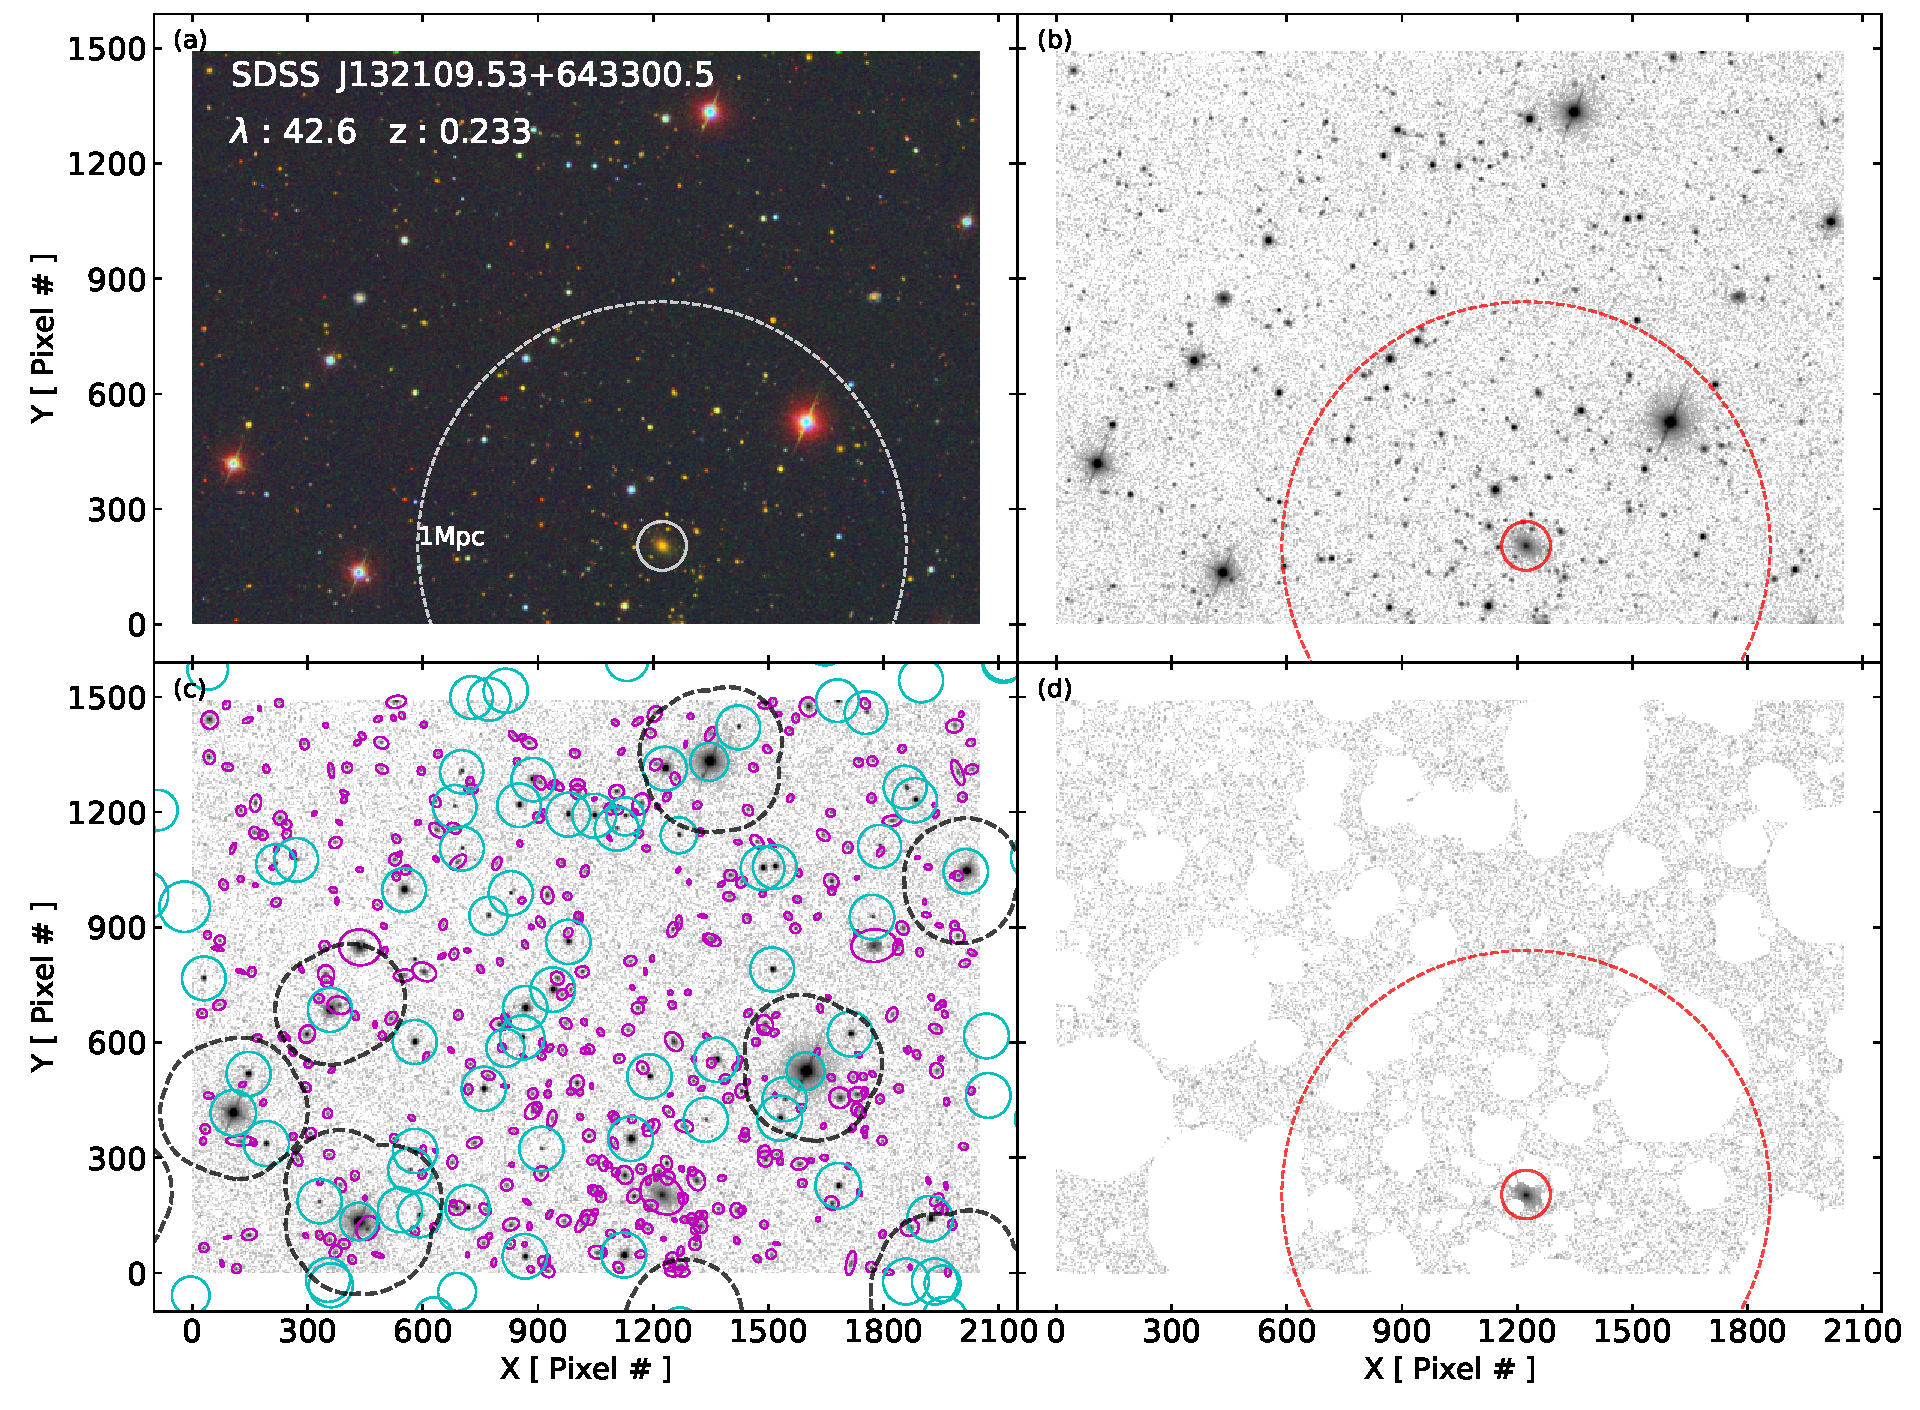
\includegraphics[width=0.96\textwidth]{fig/img_process.pdf}
\caption{Example of star and galaxy masks on the standard
    SDSS image frame ($589\times 811\,\sqarcsec$) of a cluster with
    $\lambda{=}42.6$ at $z=0.233$.\ying{change 42.611 to 42.6, and is the
    redshift 0.233 or 0.245?} \xkchen{Done!} The image dimension is $2048$ pixels by
    $1489$ pixels, and the white margin area between the image boundary and
    the panel edge has a width of $100$ pixels. Panel (a): SDSS $gri$-band
    composite image of the cluster, with its BCG indicated by the inner
    solid circle with a radius of $100\kpc$. The outer dotted circle
    indicates the cluster region of $1\mpc$ radius.  Panel (b): The SDSS
    $r$-band image frame. Panel (c): Cyan circles and magenta ellipses are
    the star and galaxy masks, respectively, while the regions delineated
    by black dashed lines are the merged masks of saturated pixels. Note
    that we also include the masks of sources that are centred in the white
    margin area (i.e., outside but close to the image boundary), as they
    could still contaminate the pixels inside the image frame. Panel (d):
    Final masked image that only includes the light from the BCG, ICL, and
    unmasked sources that are below the detection threshold.
    \label{fig:demo_mask} }
\end{figure*}


For any given set of clusters, we stack their SDSS images centred on the
BCGs and measure the average 1D SB profile from the stacked 2D image. In
this paper, we employ the observed images derived from the SDSS DR8, the
same imaging data from which the \redmapper~cluster catalogue was built.
\ying{are you sure it is DR12? The SDSS imaging survey ends at DR8} \xkchen{It is DR8.} The
images were processed with the latest SDSS photometric pipeline \xkchen{\rm{\tt{photo}}} version\xkchen{ \rm{\tt{v$5\_6$}}} \ying{need explicit name and version number of the software},
which implements an updated sky subtraction method that significantly
improves the flux estimates for bright objects, detection of faint objects
around bright objects, and extended light measurement of large objects\xkchen{\citep{Blanton2011} }.
\ying{Cite the Blanton paper} In particular, we make use of the ``corrected
frames''\ying{use proper quotation marks in LaTeX}, i.e., the calibrated
and sky-subtracted images~(with bad columns and cosmic rays interpolated
over\ying{removed or interpolated over?} \xkchen{interpolated over, $\S3.1$ in Blanton paper}). Each corrected frame has a
dimension of \xkchen{2048} pixel ${\times}$ \xkchen{1489} pixels, which corresponds to an
angular size of $13.5{\times}9.8$ arcmin$^{2}$~(the pixel size is \xkchen{$0.396$}
arcsec)\ying{shouldn't those numbers be fixed and exact? Why did you use
$\sim$?}.\xkchen{It should be! I just ignore the tail numbers, thus use `sim'} The improved photometric reduction of the SDSS images allows a
robust measurement of the large-scale, diffuse light distribution within
massive clusters, which was severely underestimated in the previous SDSS
photometric pipeline \xkchen{\citep{Bernardi2013, Kravtsov2018} }. \ying{cite the Kravtsov and Bernardi papers.}

\begin{figure*}
    \centering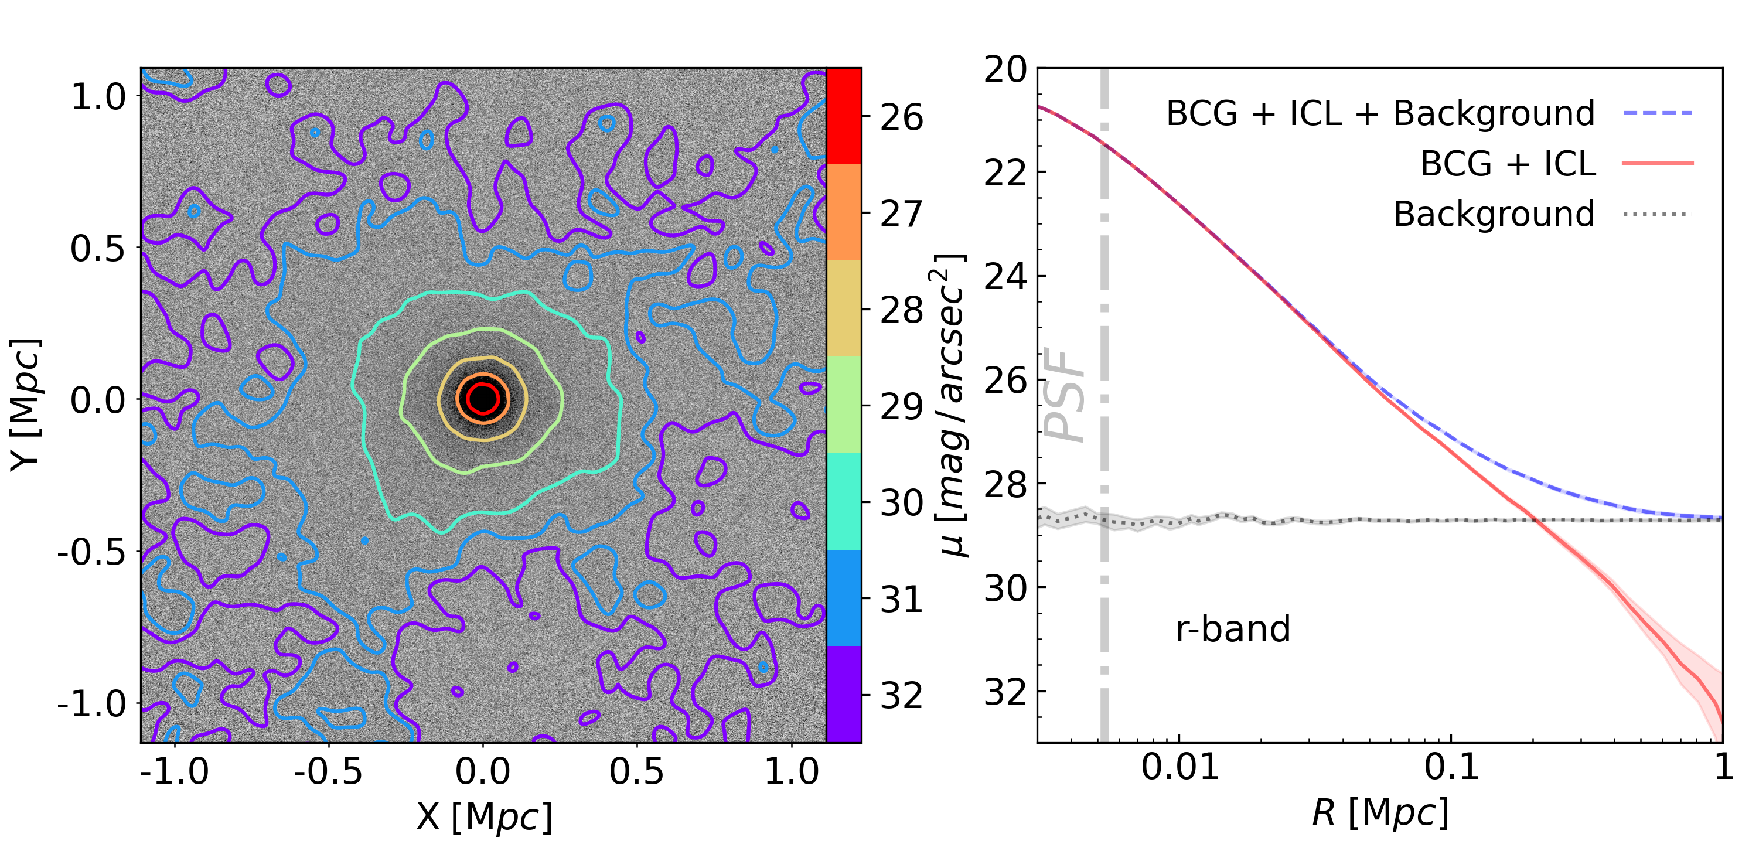
\includegraphics[width=0.96\textwidth]{fig/mass-bin_r-band_BG-sub_2D.pdf}
    \caption{{\it Left}: $r$-band stacked $2$D image of the BCG+ICL of our
    overall cluster sample (grayscale). Contour lines indicate the seven
    levels of SB ranging from $26$ to $32\,\sbmag$, colour-coded by the
    vertical colourbar.  \textit{Right}: SB profiles of the BCG+ICL
    signal~(red solid), background~(gray dotted), and the sum of the signal
    and background~(blue dashed). Shaded band centered on each curve
    indicates the $1\sigma$ uncertainties estimated from Jackknife
    resampling. \label{fig:2D_all} }
\end{figure*}


Since the stacked measurement of the outer ICL is very sensitive to image
quality, we apply a two-step procedure to identify the defect images.  In
the first step, we perform visual inspection of each image to look for
strong defects that could severely undermine the stacked signal across all
scales, e.g., extremely bright stars~(and their extended bright wings) and
strong cosmic rays across the frame. In the second step, we develop a
simple $\sigma$-clipping scheme to reject some mildly defective images that
could still impair our capability of detecting the faint ICL on scales
larger than a few hundred $\kpc$s. In particular, we divide each image
frame~(after masking out all the galaxies, bright stars, and saturated
pixels; described further below) into \xkchen{70} 200-pixel${\times}$200-pixel
cells \xkchen{(The pixel near the edge will be directly merged into the nearest cell, so the cell size of the last row and the last column will be larger than 200)}, and measure the average pixel flux ($\bar{f}_{\mathrm{cell}}$)
within each cell. In addition, we measure the
mean~($\bar{f}_{\mathrm{img}}$) and scatter~($\sigma$) of the average
fluxes of the \xkchen{70} cells, and compute the deviation of the average flux of
each cell from the mean flux of the entire image as $\Delta
f{\equiv}|\overline{f}_{\mathrm{cell}}{-}\overline{f}_{\mathrm{img}}|$. We
consider any image that includes a large block of $M$ connected cells with
$\Delta f{>}N \sigma$ to be a potential contaminant. After extensive
convergence tests, we find that the combination of \xkchen{$M{=}5$} and
\xkchen{$N{=}6$} provides an robust selection criteria for culling out bright
extended features of non-cluster origin.  In total, we identify \xkchen{1466}
strongly and \xkchen{1690} mildly defective images from all three bands and exclude
them from further stacking analysis.


\section{Surface Brightness Profile}
\label{sec:sb}


To measure the BCG+ICL SB profiles $\mubi$ via image stacking, we mask out
the bright stars and non-BCG galaxies~(i.e., satellites and background
galaxies) from each image, and then transform all the images from the
cluster redshifts to the same reference redshift of
$z_{\mathrm{ref}}{=}0.25$~(with the same pixel size but different image
sizes).


Our method of measuring the diffuse light via image stacking is largely
similar to that of \citep[hereafter referred to as \citetalias{Zibetti2005}]{Zibetti2005},
\ying{learn the citetalias command I applied earlier},\xkchen{Done!} but with two
important distinctions. Firstly, we directly utilize the sky-subtracted
corrected frames for our SB measurements, while \citetalias{Zibetti2005} performed an
independent sky subtraction on images in the SDSS Early Data Release. We
have tested the \citetalias{Zibetti2005} sky-subtraction method on the raw DR8 SDSS images and
find that the \citetalias{Zibetti2005} method generally produces consistent results compared to
the SDSS pipeline.  Secondly, we estimate the background level of the SB
profiles, primarily due to undetected background galaxies and foreground
stars, by stacking the real SDSS images centred on the coordinates of
\redmapper~random clusters, while \citetalias{Zibetti2005} inferred the background SB by
extrapolating from the best-fitting projected
Navarro-Frenk-White~(NFW)~\citeme \xkchen{\citep{Navarro1996} } profile of the SB measurement below 900
$\kpc$. We describe each step of our SB measurement in turn below.


\subsection{Image Masking}
\label{subsec:mask}

\xkchen{Present version:}
\xkchen{For each image frame, we query the full width at half maximum (FWHM) of all stars brighter than $m_r{=}20$ within ${\sim}12.53arcmin$ ($1.5$ half diagonal length of the image frame) around the center of the frame. We also query saturated pixels in each frame within the same query region. Next, we select stars that have FWHM measurement in at least one of the other two bands, and apply a mask with a diameter of $30{\times}$ the maximum FWHM among the three bands. For saturated pixels, we increase the diameter of the masks to 75$\times$FWHM in each band. We drop the stars fainter than $m_r{=}20$ to minimize the impact of the foreground signal on our ICL measurement (\citetalias{Zibetti2005}). Moreover, stars fainter than $20\,mag$ have no obvious impact on surrounding pixels and have no good photometric measurement as those bright stars. If we apply the mask on these faint stars, surrounding pixels with ICL signal surrounding may be removed, which will introduce extra uncertainty in our ICL measurement. Even if the effects of those faint stars are non-negligible, we expect that the effects of these faint stars can be systematically removed by our background subtraction, in which we apply the same image processing as the cluster catalog on images matched with the \texttt{redMaPPer} random cluster catalog.}

\xkchen{Previous version:}
For any star brighter than $m_r{=}20$, \xkchen{and have the full width at
half maximum (FWHM) measured in at least one of the other two
bands}\ying{Why in at least two? and what about those stars that only have
FWHM measured in r band only?} \xkchen{When I did the star masking, I just follow the measurement limit for stars in Z05. They don't mention why apply this limit. I think this limit is to make sure these stars are a real objects. I don't know how it will be if I use stars oberved in one specific band only.}, we measure the maximum FWHM~(full width at half maximum) of the three bands and adopt $30\times$FWHM as the diameter
of its mask. For very bright stars surrounded by a large number of
saturated pixels\ying{how did you identify those stars? by what
quantitative criteria?},\xkchen{This is a mistake, I do not identify those bright stars, I just located saturated pixels surrounding them, and the mask size is applied on saturated pixels} we increase the diameter of the masks to 75$\times$FWHM.

\xkchen{Previous version:}
\xkchen{According to \citetalias{Zibetti2005}, this magnitude limit ensures that stars are masked unlikely to be misclassified galaxies.} \ying{this sentence does not scan.} \xkchen{Stars fainter than 20mag would have no systematic effect on ICL measurement due to their random location in the
image frames, except the impacts on the signal fluctuation.}\ying{This
explanation is problematic. Both the bright and faint stars are random on
the sky.}

We have extensively tested the impact of different mask sizes on
the mesured BCG+ICL SB profile, and veried that our choices yield the best
combination of signal-to-noise ratio~(S/N) and star light mitigation.


For the galaxy masks, we run \texttt{SExtractor}\footnote{We use \href{https://github.com/astromatic/sextractor/releases}{SExtractor version 2.25.0} throughout the present work.}\citeme\xkchen{\citep{Bertin1996} } on the cluster
images in three bands separately, using a detection threshold of
$1.5\sigma$ and a minimum detection area of five pixels. Such detection
criteria result in a limiting magnitude of roughly \xkchen{22.08 in the $i$ band}~(i.e., absolute
magnitude of \xkchen{-18.49} at $z{=}0.25$), \xxx \xkchen{Here I don't find the detection limit for extended sources. The $21\,mag$ is $10{-}\sigma$ detection limit for galaxies such that the magnitude error for faintest objects is ${\sim}0.1$} deeper than the nomial SDSS
detection limit for extended sources. We mutiply the semi-major and
semi-minor radii of the ellipses detected by \texttt{SExtractor} by a
factor of eight, and adopt the augmented ellipses as the masks for
galaxies.  We include the BCGs in the masks for the image selection
described in \S\ref{subsec:img}, but leave them unmasked in the stacked
profile measurements. The factor of eight is a relatively conservative
choice, which ensures that we remove all the light physically associated
with the satellite galaxies and the scattered light from some of the very
bright, nearby galaxies.


\begin{figure*}
    \centering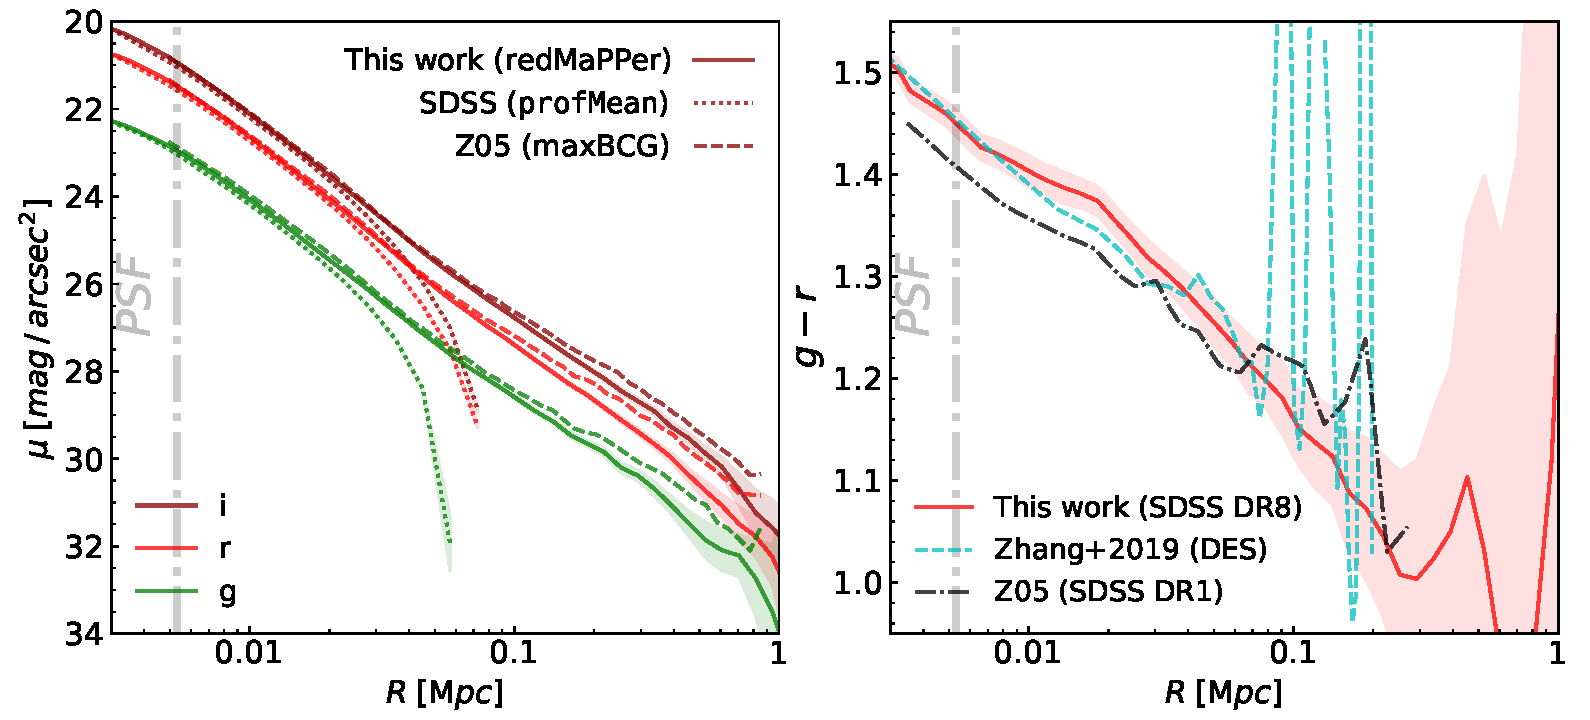
\includegraphics[width=0.96\textwidth]{fig/total_sample_compare_to_Z05.pdf}
    \caption{Comparison of our measurements of the BCG+ICL SB~(left) and
    colour~(right) profiles with previous studies. {\it Left}: Solid,
    dashed, and dotted curves indicate the BCG+ICL SB profiles from our
    measurements for \redmapper~clusters, \citetalias{Zibetti2005} for maxBCG clusters, and \xkchen{\uline{the SDSS DR7 photometric pipeline for the \redmapper~BCGs, respectively.} } \xkchen{the averaged surface brightness profile of the BCGs derived from the \texttt{profMean}\protect\footnotemark[2] (which is downloaded from the SDSS Schema Browser\protect\footnotemark[3]), respectively.}
    Green, red, and maroon curves are the measurements for the g, r, i
    bands, respectively. The gray shaded region on the left roughly
    corresponds to the scale of PSF. {\it Right}: Red solid, cyan dashed,
    and black dot-dashed curves indicate the BCG+ICL colour profiles
    measured by our work from SDSS DR8, \citetalias{Zibetti2005} from SDSS DR1, and Zhang et al.
    2019 from DES, respectively.  The red shaded band represents our
    $1\sigma$ uncertainties estimated from Jackknife resampling.
    \label{fig:Z05_comparison} }
\end{figure*}
\footnotetext[2]{Data model of \texttt{profMean}: https://www.sdss.org/dr12/algorithms/magnitudes/.}
\footnotetext[3]{SDSS Schema Browser of \href{http://skyserver.sdss.org/dr12/en/help/browser/browser.aspx\#\&\&history=search+profMean}{\texttt{profMean}}.}


To further remove any contamination induced by bright stars and extended
sources from outside the image boundaries, we identify all the \xkchen{8} images
adjacent to each target image, and apply the same masking procedure to
those neighboring images.  We then merge the external star and galaxy masks
that overlap with the target image into the internal mask. Finally, we
merge the three sets of masks from the {\it gri}-bands into a single image
mask, so that objects below the detection threshold in one particular band
but detectd in another would still be masked out in that band. By adopting
a single uniform mask across three bands, we further ensure that the
mesurement of BCG+ICL colour profiles is robust against the discrepancy in
the masks of different bandpasses..


Figure~\ref{fig:demo_mask} demonstrates the efficacy of our masking
procedure using the $r$-band corrected frame of a typical cluster in our
sample~(with $\lambda{=}42.6$ and $z{=}0.233$). Each panel has a dimension
of 2248 by 1689 pixels, larger than the orignal size of the image frame by
200 pixels on each side. Panel (a) shows the false-colour image of the
cluster, with the large dashed and small solid concentric circles
indicating 1 $\mpc$ and 100 $\kpc$-radius regions centred on the BCG,
respectively.  Panel (b) is similar to panel (a) but shows the $r$-band
image, with the grayscale indicating the individual pixel fluxes.  Panel
(c) shows the masks of the detected stars~(cyan solid circles), saturated
pixels~(black dashed circles), and galaxies~(magenta solid ellipses) within
the field. The circles within the white strips surrounding the original
image frame represent the sources from neighboring parts of the sky.
Clearly, some of the bright stars and saturated pixels in the white strips
could significantly pollute pixels of the cluster image. Finally, panel (d)
shows the final $r$-band image after all the masks have been applied,
including those derived from the $g$ and $i$-band images. We expect the
fluxes within the cluster centre to be dominated by the BCG and ICL, but
there still exist some unmasked satellite galaxies, faint background
galaxes, and faint foreground stars in the final image of panel (d). We
will statistically remove the contamination in the BCG+ICL profiles by the
undetected~(hence unmasked) backgroud sources in \S\ref{subsec:sbprofile}
and faint satellites in \S\ref{subsec:budget}.


\subsection{Image Rescaling to Reference Redshift}
\label{subsec:rescale}


To stack images at the same physical scale, we transform all the masked
images to the reference redshift $z_{\mathrm{ref}}{=}0.25$ with the same
pixel size. Firstly, we rescale the pixel size of each image by the square
of the angular diameter distance ratio between the observed and reference
redshifts, $(D_A^{\mathrm{obs}}/D_A^{\mathrm{ref}})^2$, and the flux within
the pixel by the square of the ratio between the two luminosity distances,
$(D_L^{\mathrm{obs}}/D_L^{\mathrm{ref}})^{2}$. Cosmic dimming is
automatically included as the pixel SB varies by
$[(1+z_{\mathrm{obs}})/(1+z_{\mathrm{ref}})]^4$. We do not apply any
K-correction to the cluster fluxes due to the lack of robust SED templates
for the ICL. However, since the reference redshift is close to the median
redshift of the sample, we anticipate that the amount of K-correction in
the stacked images should be largely cancelled out. In addition, we correct
for Galactic extinction on the stacked profiles, rather than the individual
images. Secondly, we resample all the rescaled images to $0.395''$\xkchen{$0.396''$} per
pixel resolution, i.e., the original pixel size of the SDSS images. We then
redistribute the image fluxes into the resampled pixels, so that the flux
in each new pixel is $\Sigma \mu_i A_{i}$, where $\mu_i$ is the SB of the
$i$-th pixel in the rescaled image and $A_{i}$ is the overlapped area
between pixel $i$ and that new pixel.



\subsection{BCG+ICL SB Profile Measurement}
\label{subsec:sbprofile}

\begin{figure}
    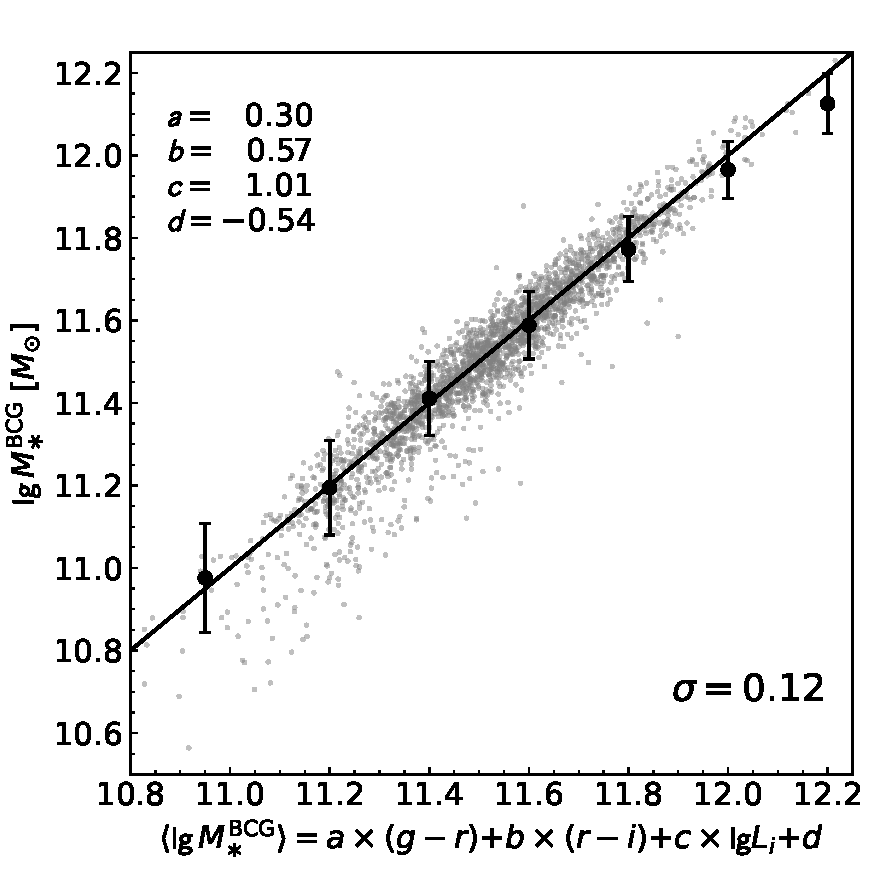
\includegraphics[width=0.48\textwidth]{fig/Mass-to-Li_estimation.pdf}
    \caption{Comparison between the stellar mass-to-light ratio of BCGs
    measured from SPS modeling (y-axis) and that predicted by our linear
    estimator (x-axis). Black circles with errorbars indicate the median
    relation with its scatter, in good agreement with the one-to-one
    relation (black line). The parameters of the linear estimator are
    listed in the bottom right corner.
    \ying{change 0.302 to 0.30, and likewise for the rest} \xkchen{Done!}
    \label{fig:func_M2L} }
\end{figure}


With all clusters shifted to the reference redshift, we now stack their
images centred on the BCGs in physical coordinates. We carefully account
for the masked regions and adopt the mean flux at each pixel for the
stacked image. A total SB profile is then computed as the azimuthally
averaged SB within each annulus. However, this total SB profile includes
not only the light from the BCG+ICL, but also contributions from the
unmasked satellite galaxies, background galaxies, and foreground
stars~(i.e., BCG+ICL+Background). We will estimate the unmasked satellite
contribution by inspecting the satellite stellar mass functions later in
\S\ref{subsec:budget}, and describe the removal of the background SB
induced by the other two components below.



For any given set of clusters, we select a matching sample of random
clusters with the same joint distribution of redshift and richness from the
SDSS \redmapper~random catalogue~(v6.3) \xkchen{\citep{Rykoff2016}}.\ying{find the reference to the
random catalogue and describe it accordingly} \xkchen{Specifically, \citep{Rykoff2016} did this by sampling fake clusters across the entire survey volume, which shares the same richness and redshift distribution as the true cluster catalog. Firstly, pairs of {($\lambda,\,z_{\lambda}$)} are randomly sampled from the data catalog. These pairs are assigned to a random position ($\alpha,\,\delta$). At this step, the selected $z_{\lambda}$ is compared to the maximum redshift at which the cluster can be detected (details in $\S3$ of \citep{Rykoff2016}). This procedure will be repeated with new ($\alpha,\,\delta$) in each time until the $z_{\lambda}$ is smaller than the maximum redshift at the random position. Each cluster was sampled about $n_{\mathrm{samp}}{\sim}1000$ times to avoid the impact of noise in the random catalog on correlation measurements made on it. Thirdly, local mask fraction $f_{mask}$ and scale factor $\lambda / S$ are estimated based on the depth map and footprint mask. Only random points with $f_{mask}\leq0.2$ and $\lambda / S \geq20$ are left (simply as $n_{\mathrm{keep}}$), and weighted with the factor $\omega=n_{\mathrm{samp}}/n_{\mathrm{keep}}$ (avoiding the impacts of survey boundary, masks, and depth variation on random points).}
Since the sensitivity of \redmapper~algorithm to the background is incorporated in the generation of
random clusters, we expect the backgroud SB of the random cluster images to
be similar to that of the observed ones. To measure the background SB
profile, we download the SDSS corrected frames that host the random
clusters, and perform the same two-step quality inspection to remove defect
images from the random sample. We then apply the same masking, rescaling,
and stacking procedures to the random cluster images that pass the
inspection, thereby producing a background SB profile for the clusters. We
repeat such procedure ten times by reshuffling the relative positions of
the BCGs on the images after each measurement, and calculate the average of
the ten measurements as our the final background SB profile.



Finally, we derive the BCG+ICL SB profile $\mubi(R)$ by subtracting the
background SB profile from the total SB profile. We further normalise the
$\mubi(R)$ profile to be zero at projected distance $R{=}2\,\mpc$, and
focus on the SB signals at $R{<}1\,\mpc$ for the rest of the paper. Note
that the $\mubi(R)$ profile measured in this way includes the contribution
from the faint satellite galaxies that are unmasked. We do not subtract
this contribution from our measured $\mubi(R)$ and $\sigbi(R)$ profiles,
but will nonetheless estimate the total stellar mass of the unmasked
satellites $\Sigma M_*^{\mathrm{unmasked}}$ in \S\ref{subsec:budget}.  In
order to estimate the uncertainties of $\mubi(R)$, we employ the standard
Jackknife resampling technique by dividing each cluster sample into 30
equal-size subsamples, and compute the error matrix from the 30
``leave-one-out'' measurements~\citeme \xkchen{\citep{Efron1981, Efron1982} }. \ying{need a few sentences
describing the comparison with the Z05 error measurements}
\xkchen{In \citetalias{Zibetti2005}, they estimate the uncertainty of measurement by the rms in each radial bin. Specifically, they divided each annulus into $n$ sectors with aperture angle $\theta\simeq\Delta R /R$, then used the rms among those sectors to estimate the statistical error on their average surface brightness as $\mathrm{rms}/\sqrt{n-1}$. Comparing \citetalias{Zibetti2005} error to the estimation in this work, \citetalias{Zibetti2005} estimation is slightly higher within ${\sim}10\,\kpc$ but lower beyond ${\sim}10\,\kpc$. The pixel number at central radii is not enough to have a good angular sector division. At radii beyond ${\sim}10\,\kpc$, error estimation in this work is higher than \citetalias{Zibetti2005} ${\sim}1$ to $2$ times. This difference is mainly because that \citetalias{Zibetti2005} estimation reflects the fluctuation in each annulus of the stacked image, while estimation in this work indicates the scatter among the 30 subsamples. Although the fraction of different images in subsamples is only a few percent, the signal beyond BCG boundaries is so weak that scatter among subsamples is larger than the fluctuation in the stacked image.}



Figure~\ref{fig:2D_all} shows the stacked 2D image of the BCG+ICL SB
distribution~(left) and the corresponding SB profiles~(right) for our
overall cluster sample in the $r$ band. In the left panel, the grayscale
intensity represents the SB of each pixel, while the contour lines indicate
seven levels of SB ranging from $\mu=26\,\sbmag$ at $R{\simeq}50\,\kpc$ to
$32\,\sbmag$ at $R{\simeq}1\,\mpc$~(with $\Delta \mu=1\,\sbmag$ increasing
outwards), colour-coded by the vertical colorbar on the right. The
azimuthally averaged 1D SB profiles are shown in the right panel, where the
blue dashed, gray dotted, and red solid curves indicate the total stacked
SB~(BCG+ICL+background), background SB, and the BCG+ICL SB profiles
$\mubi$, respectively. The shaded bands indicate the SB uncertainties
estimated from Jackknife resampling. Thanks to the large sample size, we
are able to robustly measure the diffuse cluster light down to roughly
$32\,\sbmag$ at $R{=}1\,\mpc$ despite the relatively shallow depth of the
SDSS imaging~($\xxx\sbmag$\xkchen{$22.54\sbmag$ in the $i$ band}).


We compare our BCG+ICL SB~(left) and g-r colour~(right) profiles with the
results from previous studies in Figure~\ref{fig:Z05_comparison}. In the
left panel, solid and dashed curves indicate the $\mubi(R)$ profiles
meausured for the \redmapper~clusters in this work and the maxBCG \xkchen{\citep{Annis1999, Bahcall2003} } clusters
by \citetalias{Zibetti2005}~\ying{cite maxbcg}, respectively, in the SDSS $g$~(green),
$r$~(red), and $i$~(maroon) bands.  The ampliutdes of the maxBCG profiles
are slightly higher than the \redmapper~ones on all scales, likely because
the maxBCG clusters selected by \citetalias{Zibetti2005} are on average higher mass systems than
ours. On small scales, our stacked profiles are consistent with the average
BCG light profiles~(dotted) derived by the SDSS photometric
pipeline \xkchen{\it{\rm{ photo v$5\_6$} } } \ying{name and version number}, but the dotted curves are rapidly
cut off on scales above 30 $\kpc$, due to the over-subtraction of the sky
background on relevant scales~\citeme \xkchen{\citep{Blanton2011, Aihara2011} } \xkchen{I think this may be not due to sky subtraction, or sky subtraction is not the majority. In Aihara's paper, they compare the photometric measurement on bright galaxies(i.e. the effective radius and magnitude), and they found that the improvement of the DR8 version pipeline does not work well on bright galaxies. The poor deblender may assign some of the light in the outer parts of bright galaxies to superposed fainter stars and galaxies}. For the $g{-}r$ color profiles shown
in the right panel, our measurement~(red solid) is slightly redder than the
that of \citetalias{Zibetti2005}~(black dot-dashed), consistently with the \citetalias{Zibetti2005} BCGs being more
massive.\ying{have you corrected for reddening here?} \xkchen{Yes} We also show the DES
g-r color profile measured by Zhang et al. 2019\citeme \xkchen{\citep{Zhang2019} }  for the DES
clusters~(cyan dashed), which exhibits a simialr slope compared to \citetalias{Zibetti2005} and
our results. The Zhang et al. profile is measured from a much smaller
cluster sample than ours with \xkchen{$\sim280$} DES redMaPPer clusters, therefore their
measurements are cut off at \xkchen{200} $\kpc$ despite the DES photometry is
roughly \xkchen{2} magnitudes deeper than SDSS.


\section{Stellar Surface Density Profile}
\label{sec:sigma}

\subsection{Mass-to-Light Ratio}
\label{subsec:moverl}

\begin{figure*}
    \centering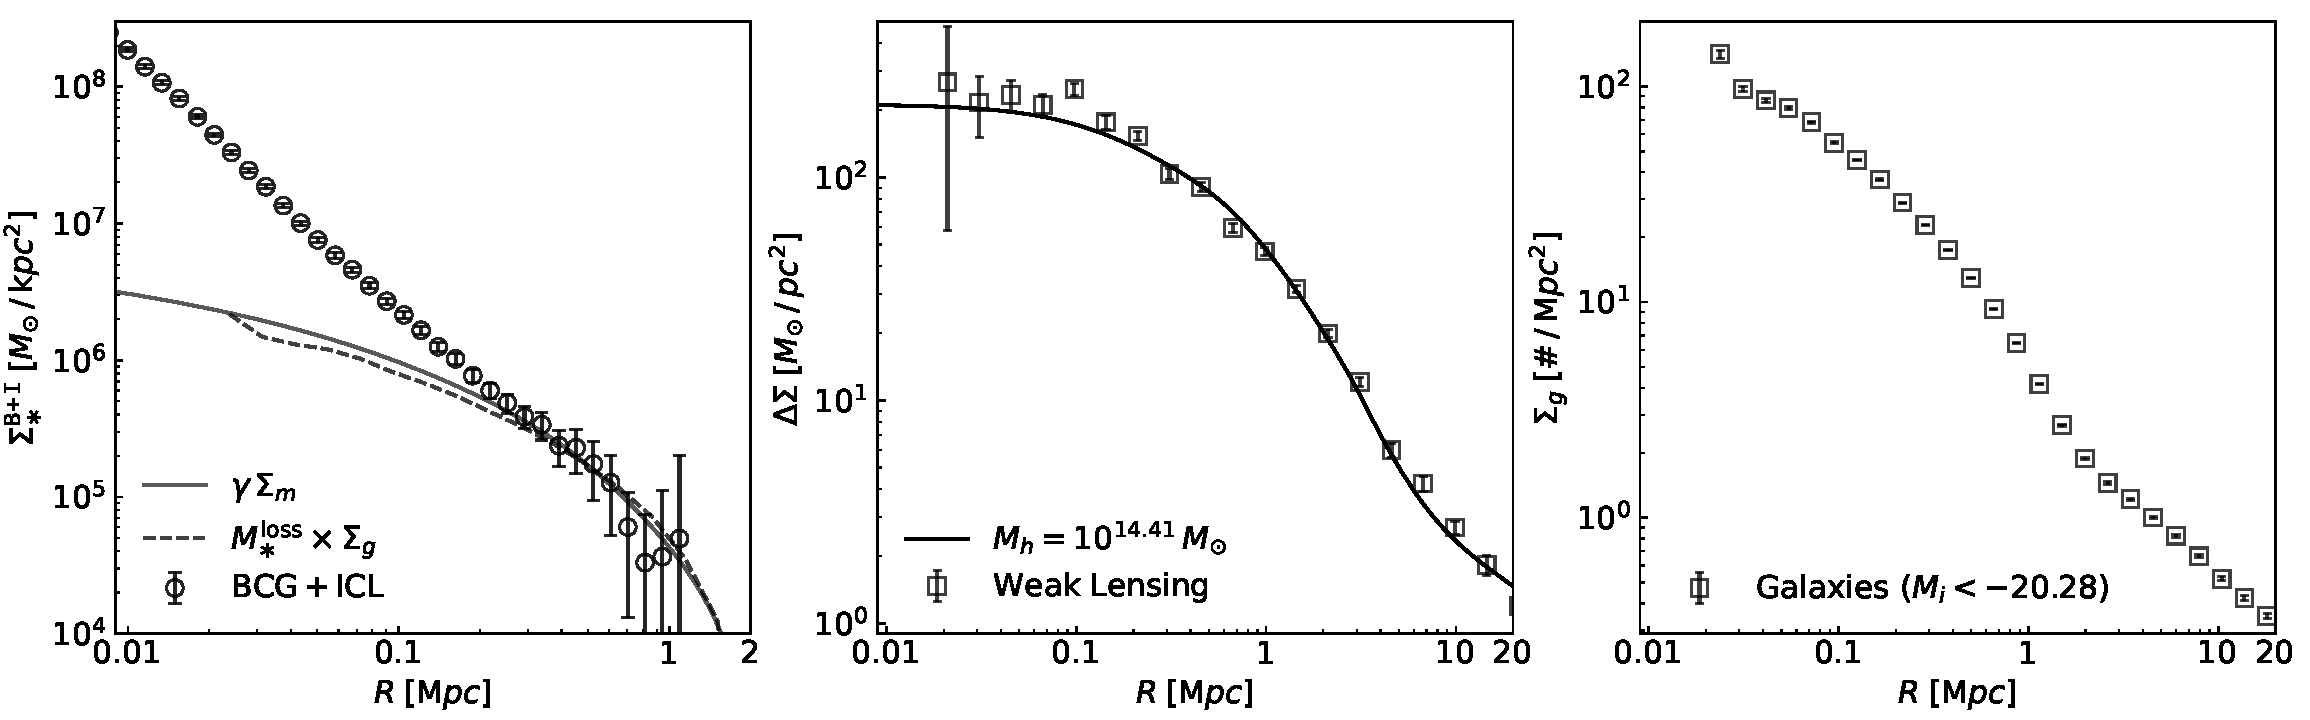
\includegraphics[width=0.96\textwidth]{fig/total_sample_SB_SM.pdf}
    \caption{{\it Left}: Stellar surface mass density profiles. Open
    circles with errorbars are the $\sigbi(R)$ profile measured in this
    work, while solid~($\gamma\sigm$) and dashed
    black~($M_*^{\mathrm{loss}}\sigg$) curves are the model predictions
    assuming that the outer ICL follows the distributions of dark
    matter~(middle panel) and satellite galaxies~(right panel),
    respectively.  {\it Middle}: Surface density contrast $\ds(R)$ measured
    by weak lensing~(squares with errorbars) and predicted by the
    best--fitting model described in \citetalias{Zu2021}. {\it Right}:
    Galaxy surface number density profile $\sigg(R)$ measured from the
    cluster-galaxy cross-correlation funtion.\ying{-20.276 to -20.28} \xkchen{Done!}
    \label{fig:massprof3panel} }
\end{figure*}

For each cluster sample, we now convert the light profiles $\mubi$ measured
in three bands into a BCG+ICL stellar surface density profile $\sigbi$
using an empirical method based on the template fitting described
in~\S\ref{subsec:cls}.  In particular, we assume the $i$-band mass-to-light
ratio~($M_*/L_i$) can be described by a simple linear function of the
$i$-band luminosity $L_i$, g-r, and r-i colours,
\begin{equation}
    \lg(M_{\ast}/L_{i}) = a \cdot (g-r) + b \cdot (r-i) + (c - 1) \cdot \lg L_{i} + d.
    \label{eqn:moverl}
\end{equation}
We use $\msbcg$, i-band cModel magnitudes, and the model magnitude colors
of the BCGs to infer the values of $\{a, b, c, d\}$ via least-square
fitting. Figure~\ref{fig:func_M2L} demonstrates the efficacy of our
empirical calibration of $M_*/L_i$, where we show the distribution of BCGs
on the observed vs. predicted $\msbcg$ plane. Filled circles with errorbars
indicate the mean observed $\msbcg$ at fixed $\langle\msbcg\rangle$
predicted by Equation~\ref{eqn:moverl} with $\{a{=}0.30, b{=}0.57,
c{=}1.01, d{=}{-}0.54\}$, in good agreement with the one-to-one
relation~(solid line). The outliers in the bottom left corner mainly
consist of BCGs with relatively blue colours, which have minimal impact on
the least-square fit due to their small fraction.


\subsection{Surface Density Profiles of Diffuse Light, Dark Matter, and Satellite Galaxies}
\label{subsec:sigmathree}

In the left panel of Figure~\ref{fig:massprof3panel}, we apply our
best--fitting formula of $M_*/L_i$~(Equation~\ref{eqn:moverl}) to the $gri$
SB profiles in Figure~\ref{fig:Z05_comparison} and derive the BCG+ICL
stellar surface density profile $\sigbi(R)$ for the overall cluster sample,
as shown by the open circles with errorbars. Clearly, the $\sigbi$ profile
has a significant ICL component that extends to a few ${\times}10^4
\msol\kpc^{-2}$ at scales ${\sim}500\,\kpc{-}1\,\mpc$, where we expect that
the ICL largely follows the distributions of dark matter and satellite
galaxies. To compare the surface density profile of the diffuse component
with that of the dark matter and satellite galaxies, we show the
measurements of cluster weak lensing $\ds$ and galaxy number density
profile $\sigg$ for
the overall sample in the middle and right panels of
Figure~\ref{fig:massprof3panel}, respectively~(squares with errorbars).


We obtain the $\ds$ and $\sigg$ measurements~(as well as the theoretical
model of $\ds$) by faithfully following the methods described in
\citetalias{Zu2021}.  Briefly, the surface density contrast profile
$\ds(R)$ is measured from weak lensing using the DECaLs DR8 imaging, while
the galaxy surface number density profile $\sigg(R)$ is calculated by
cross-correlating clusters with the photometric galaxies within SDSS
DR8~\xkchen{(Mag$_i{<}-20.28$)}. We also show the best-fitting $\ds(R)$ profile
predicted by the theoretical model of \citetalias{Zu2021} in the middle
panel~(solid curve), which describes the small-scale lensing using an NFW
halo density profile with the cluster miscentring effect constrained by
X-ray observations, and the large-scale lensing using a biased version of
the matter clustering. From the $\ds$ modelling, we infer the average halo
mass of our cluster sample to be $\mh{=}\xxx$\xkchen{$\mh{=}10^{14.41}\,\msol$}, consistent with the results
from \citetalias{Zu2021}.  We refer interested readers to
\citetalias{Zu2021} for technical details that are beyond the scope of this
paper.



Returning to the left panel of Figure~\ref{fig:massprof3panel}.  Solid and
dashed curves show the matter surface density profile $\sigm$ and galaxy
surface number density profile $\sigg$, multiplied by a scale factor
$\gamma$ and the average mass loss per galaxy
\xkchen{$M_*^{\mathrm{loss}}=10^{10.2}\msol$}, respectively. In particular, the scale
fator is defined as
\begin{equation}
    \gamma(R) = \frac{\Sigma_{\mathrm{ICL}}(R) +
    \Sigma^{\mathrm{unmasked}}_{\mathrm{sat}}(R)}{\sigm(R)}
    \label{eqn:gamma}
\end{equation}
where $\Sigma_{\mathrm{ICL}}$ is the ICL stellar mass profile and
$\Sigma^{\mathrm{unmasked}}_{\mathrm{sat}}$ is the stellar mass profile of
the unmasked satellite galaxies. By assuming that both the ICL and unmasked
satellites follow the distribution of dark matter, the above equation can
be simplied as
\begin{equation}
    \gamma(R)\equiv \gamma =f_{\mathrm{ICL}} + f^{\mathrm{unmasked}}_{\mathrm{sat}},
    \label{eqn:gamma2}
\end{equation}
where $f_{\mathrm{ICL}}$ and $f^{\mathrm{unmasked}}_{\mathrm{sat}}$ are the
ICL and unmasked satellite stellar-to-halo mass ratios, respectively.  We
infer the best-fitting values of \xkchen{$\gamma=1/419$} and
$\lg\,M_*^{\mathrm{loss}}=11.1$ by matching the scaled profiles to the
$\sigbi(R)$ measurements above $R=400\kpc$.  We will infer the values of
$f_{\mathrm{ICL}}$ and $f_{\mathrm{unmasked}}^{\mathrm{sat}}$ separately in
\S\ref{subsec:budget}.  Note that we predict the $\sigm$ profile from the
best-fitting $\ds$ model curve in the middle panel, and directly adopt the
observed $\sigg$ profile in the right panel.  Additionally, both curves are
normalized to have zero amplitudes at $R{=}2\mpc$, following the same
practice when measuring $\sigbi$.


Overall, the two scaled profiles $\gamma\sigm$ and
$M_*^{\mathrm{loss}}\sigg$ in the left panel of
Figure~\ref{fig:massprof3panel} provide good descriptions to the BCG+ICL
stellar surface density profiles at $R>400\kpc$, indicating that the ICL in
the outer region of clusters indeed follows the distribution of the dark
matter and satellite galaxies. This is consistent with the findings from
\citeme \xkchen{\citep{Montes2019, Zhang2019} }, which suggested that the ICL is an excellent tracer of dark
matter, as well as satellite stripping being the dominant channel of ICL
production~\citeme \xkchen{\citep{Montes2018, JimenezTeja2019, DeMaio2015, DeMaio2018} }. In particular, we find that our observation of the diffuse light on scales above $400\kpc$ can be explained if
$\sim$0.1{-}0.2\% of the total mass is in the form of ICL, and if
${\sim}10^{10}\msol$ of stars were stripped from each satellite galaxy into
the ICL.


\subsection{Decomposition of the BCG+ICL Surface Stellar Mass Profile}
\label{subsec:decomposition}

\begin{figure}
    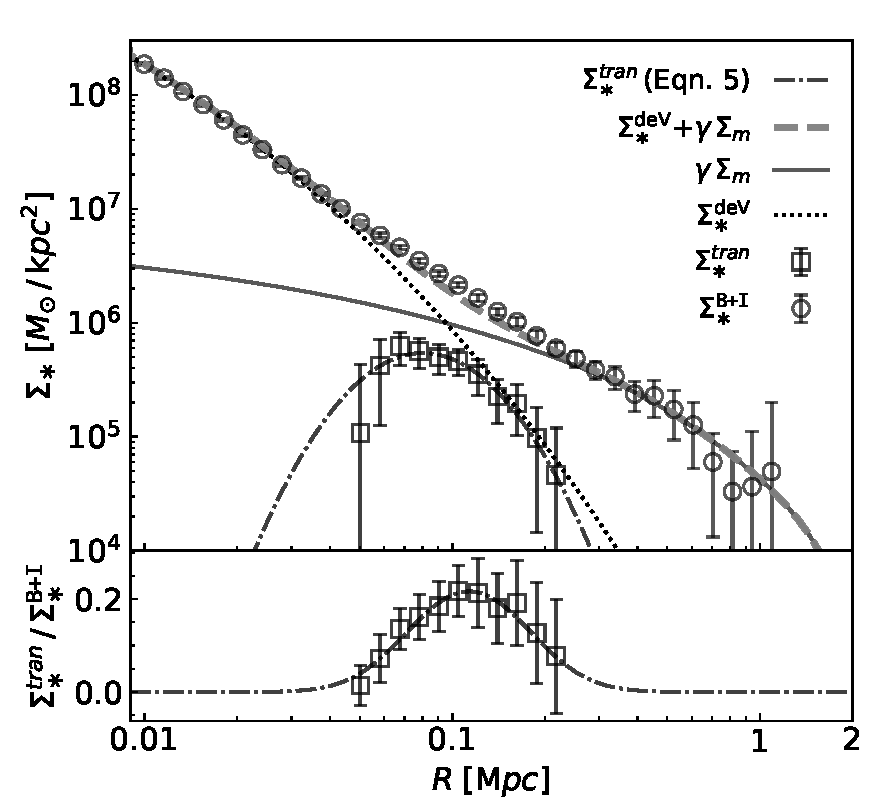
\includegraphics[width=0.48\textwidth]{fig/DM_Ng_compare.pdf}
    \caption{Decomposition of the BCG+ICL stellar surface mass density
    profile $\sigbi$~(filled circles with errobars). Solid curve is the
    total surface mass density profile $\sigm$, scaled by a scale factor
    $\gamma{\equiv}1/419$~(Equation~\ref{eqn:gamma}), while the
    best-fitting de Vaucouleurs profile for the $\sigbi$ profile at
    \xkchen{$R<20\kpc$} is shown as the dotted curve.  The sum of $\gamma\sigm$ and
    $\sigdev$ is indicated by the dashed curve, revealing an excess mass in
    the observed $\sigbi$ profile on transitional scales of
    $R{=}50{-}200\kpc$. Open circles with errorbars indicate this
    transitional component $\sigtr$, which can be described by a Log-normal
    function~(Equation~\ref{eqn:sigtr};
    dot-dashed).\label{fig:decomposition} }
\end{figure}


Given that the outer region of the ICL roughly follows the distribution of
dark matter, we can separate the observed BCG+ICL stellar surface mass
profile $\sigbi$ into at least two physicallly distinct components,
including one that follows the dark matter on large
scales~($R{=}400\kpc{-}1\mpc$) and the other BCG-dominated portion on small
scales~(\xkchen{$R{<}20\kpc$}). By further assuming that the {\it intrinsic} BCG
can be described by a de Vaucouleurs' profile, the BCG-dominated portion
may include a third component on transitional scales where the extended BCG
envelope unfolds into the ICL. Following this philosophy, we can decompose
the $\sigbi$ profile via the following three steps. Firstly, we adopt the
total surface mass profile $\sigm$ inferred from weak lensing, and
mulitiply it by \xkchen{$\gamma=1/419$} to
describe $\sigbi$ at $R>400\kpc$, as was done in the left panel of
Figure~\ref{fig:massprof3panel}.
\begin{equation}
    \Sigma_*^{\mathrm{ICL}}(R) = \gamma \sigm(R).
    \label{eqn:sigmaicl}
\end{equation}
Secondly, we fit a de Vaucouleurs' profile to the $\sigbi$ measurement on
scales below \xkchen{$R{=}20\kpc$},
\begin{equation}
    \sigdev(R) = \xkchen{ \Sigma_{e} \, exp \{ -\beta_{n} (\frac{R}{R_{e}})^{1/n} + \beta_{n} \} }.
    \label{eqn:sigmabcg}
\end{equation}
\xkchen{Where $\Sigma_{e}$ is the amplitude of surface mass profile, $n{=}4$ is the index, and $\beta_{n}{=}2\,n-0.324$. $R_{e}$ is the effective radius. For the entire cluster sample, $\Sigma_{e}{=}10^{7.92}\msol$ and $R_{e}{=}15.4\kpc$}
Finally, we subtract $\Sigma_*^{\mathrm{ICL}}$ and $\sigdev$ from the
measured $\sigbi$ profile, leaving us the transitional component
\begin{equation}
    \sigtr(R) = \Sigma_*^{\mathrm{BCG+ICL}}(R) -
    \left[\Sigma_*^{\mathrm{deV}}(R) + \Sigma_*^{\mathrm{ICL}}(R)\right].
    \label{eqn:sigmatran}
\end{equation}
Therefore, $\sigtr(R)$ represents the excess component in the diffuse light
that cannot be described by the sum of a de Vaucouleurs' profile and an ICL
mass profile that follows the dark matter.



Figure~\ref{fig:decomposition} illustrates the physical decomposition of
our observed $\sigbi$ profile~(filled circles with errorbars) into three
distinct components: a de Vaucouleurs' profile $\sigdev$~(dotted curve), a
scaled dark matter profile~$\sigicl$~(solid curve), and a transitional
component~$\sigtr$~(open circles with errorbars).  The errorbars of
$\sigtr$ are inherited from that of the $\sigbi$ measurement, assuming zero
uncertainties from the subtraction. Additionally, dashed curve indicates
the sum of the de Vaucouleurs' profile and the scaled dark matter profile,
which clearly under-predicts the signal on scales betwen $50\kpc$ and
$200\kpc$ --- a third component $\sigtr$ is required to fully describe the
diffuse light.  The ratio profile between $\sigtr(R)$ and $\sigbi(R)$ is
shown in the bottom panel of Figure~\ref{fig:decomposition}. The
transitional component accounts for more than 10\% of the total diffuse
mass on scales between $50\kpc$ and $300\kpc$, and the ratio peaks
at 35\% around $100\kpc$.
We have tested the robustness of $\sigtr(R)$ by fitting the de Vaucouleurs'
profile to a larger radius at $R=30\kpc$ or allowing the {\it sersic} index
to vary, and the centroid and amplitude of $\sigtr(R)$ are insensitive to
those changes. \ying{check this} \xkchen{On going!}


Finally, the $\sigtr(R)$ profile can be conveniently described by a
Log-normal function:
\begin{equation}
    \sigtr(R) =  \frac{\Sigma_{0}}{R \, \sigma_t \,
    \sqrt{2 \pi} } \exp \big{ \{ } - \frac{(\ln R - \ln R_t)^2} {2
    \, \sigma_t^2} \big{ \} },
    \label{eqn:sigtr}
\end{equation}
where \xkchen{$\sigma_t{=}0.45$} and \xkchen{$R_t{=}98.03\kpc$} are the characteristic log-width
and centroid of the transitional component, respectively.\ying{refit the
data using the new parametrization} \xkchen{On going!} The best-fitting
Equation~\ref{eqn:sigtr} is shown as the dot-dashed curves in both panels
of Figure~\ref{fig:decomposition}. Although our decomposition method is
physically-motivated, it depends strongly on the assumptions that the inner
BCG is strictly de Vaucouleurs and the outer ICL follows the dark matter.
In future work, we will investigate if a similar transitional component
would emerge from the hydrosimulations after we apply our decomposition
method to the simulated clusters.


\subsection{Stellar Mass Budget of Clusters}
\label{subsec:budget}

\begin{figure}
    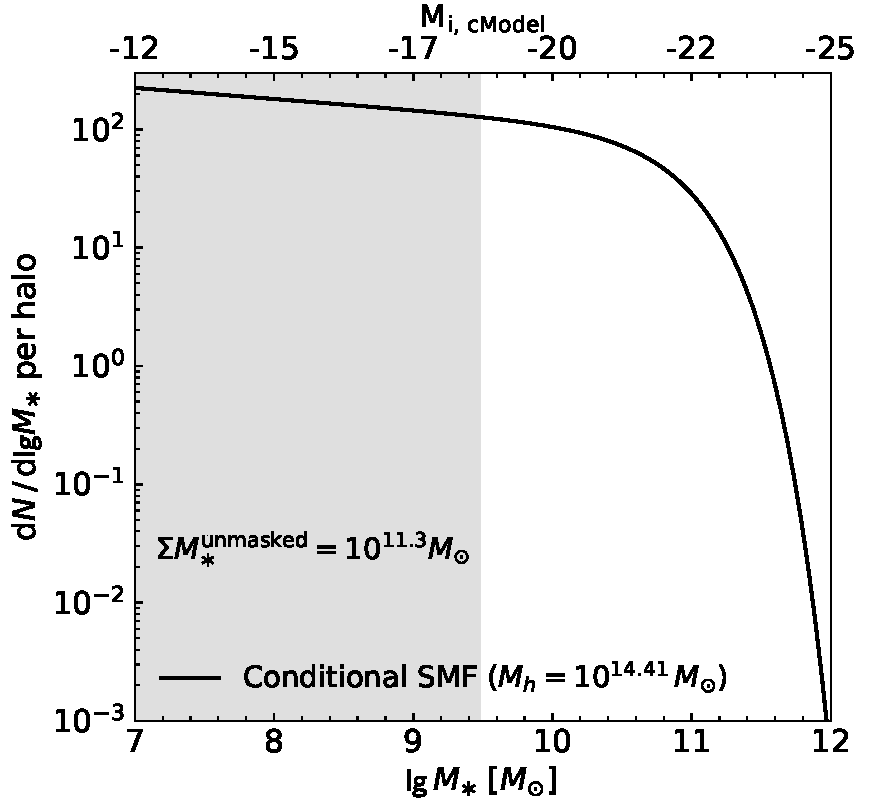
\includegraphics[width=0.48\textwidth]{fig/sat_icl_mass_estimation.pdf}
    \caption{Conditional satellite stellar mass function of our cluster
    sample~(solid curve). Gray shaded region indicates the stellar mass
    range of satellites that are undetected by our source finding
    algorithm~(hence unmasked). The top x-axis indicates the corresponding
    $i$-band cModel absolute magnitudes. The total stellar mass of the
    unmasked satellite galaxies is $\Sigma M_*^{\mathrm{unmasked}}=2\times
    10^{11}\msol$. \label{fig:csmf} }
\end{figure}


With the physical decomposition in Figure~\ref{fig:decomposition}, we are
now ready to derive the stellar mass budget of clusters in three states:
BCG, ICL, and satellite galaxies. In order to estimate the total amount of
stellar mass inside the satellite galaxies, we make use of the conditional
stellar mass function~(CSMF) of clusters measured by Yang et al.
2012~\citeme \xkchen{\citep{Yang2012} }.  In particular, we adopt the shape of the measured CSMF for
the halo mass bin of \xkchen{$10^{14.37}{-}10^{14.67}\,M_{\odot}$}, which can be
described by a Schechter function
\begin{equation}
  \Phi(M_{\ast}) = \phi_{ \mathrm{pivot} } \big{(} \frac{ M_{\ast} }{ M_{
      \mathrm{pivot} } } \big{)}^{\alpha+1} \mathrm{exp} \big{ \{ } -
  \frac{M_{\ast}}{M_{ \mathrm{pivot} } } \big{ \} }
    \label{eqn:csmf}
\end{equation}
with \xkchen{ $\lg M_{\mathrm{pivot}}{=}10.92\,\msol$} \ying{unit?} and $\alpha{=}-1.093$.
However, the Yang et al. CSMF was measured for a sample of galaxy groups at
$z{<}0.1$, which has a different value of $\phi_{\mathrm{pivot}}$ than that
of our cluster sample at $z{\sim}0.25$. To determine
$\phi_{\mathrm{pivot}}$, we compute the total number of satellite galaxies
per halo above our $i$-band absolute magnitude limit of \xkchen{-20.28} by integrating
the galaxy surface number density profile $\Sigma_g$ to \xkchen{$R{=}1.47\mpc$} \xkchen{(which is the median $R_{200m}$ of cluster sample. Here we estimated $R_{200m}$ based on the Mass-richness relation derived by \citep{Simet2017})}, as
shown in the right panel of Figure~\ref{fig:massprof3panel}. Given that the
$i$-band magnitude of \xkchen{-20.28} roughly corresponds to a steller mass of
\xkchen{$10^{10.2}\,\msol$}~(assuming a $M_*/L_i$ of \xkchen{1.88}), we normalise Equation~\ref{eqn:csmf}
for our cluster sample by enforcing the total number of satellites above
\xkchen{$M_*=10^{10.2}\,\msol$} to be \xkchen{57} per halo, yielding a
\xkchen{$\phi_{\mathrm{pivot}}{=}97.2\,per\,dex\,per\,\mathrm{halo}$}.\ying{unit?} Figure~\ref{fig:csmf} shows
the correctly normalized CSMF of our cluster sample~(solid curve), which we
integrate from \xkchen{$M_*{=}10^{9.47}\,\msol$} to \xkchen{$10^{12}\,\msol$} to obtain the average stellar mass of
the satellites \xkchen{$\langle{M_*^{\mathrm{sat}}}\rangle{=}10^{10.41}\,\msol$} and the total
amount of satellite stellar mass \xkchen{$\Sigma M_*^{\mathrm{sat}}{=}10^{12.55}\,\msol$}.


Furthermore, the gray shaded region~(below \xkchen{$\lg\,M_*{=}9.47$}) in
Figure~\ref{fig:csmf} indicates the stellar mass range that is below the
detection threshold of our source finding algorithm, hence unmasked during
the SB measurement.  This detection threshold roughly corresponds to the
i-band limiting cModel magnitude of \xkchen{22.08} at \xkchen{$z\sim0.25$}, i.e., an absolute
magnitude of \xkchen{-18.49}, yielding a total unmasked stellar mass of $\Sigma
M_*^{\mathrm{unmasked}}{=}2\times10^{11}\msol$.  We remove this unmasked
stellar mass contribution from the ICL stellar mass budget as follows.  The
unmasked satellite mass fraction is
\xkchen{$f^{\mathrm{unmasked}}_{\mathrm{sat}}=\Sigma
M_*^{\mathrm{unmasked}}/M_h=0.059\%$}. Since the scale factor defined in
Equation~\ref{eqn:gamma2} is \xkchen{$\gamma=1/419$}, we can infer the ICL mass
fraction as \xkchen{$f_{\mathrm{ICL}}=\gamma -
f^{\mathrm{unmasked}}_{\mathrm{sat}}= 1/419 - 0.00059 = 1/556$}.


\begin{figure}
    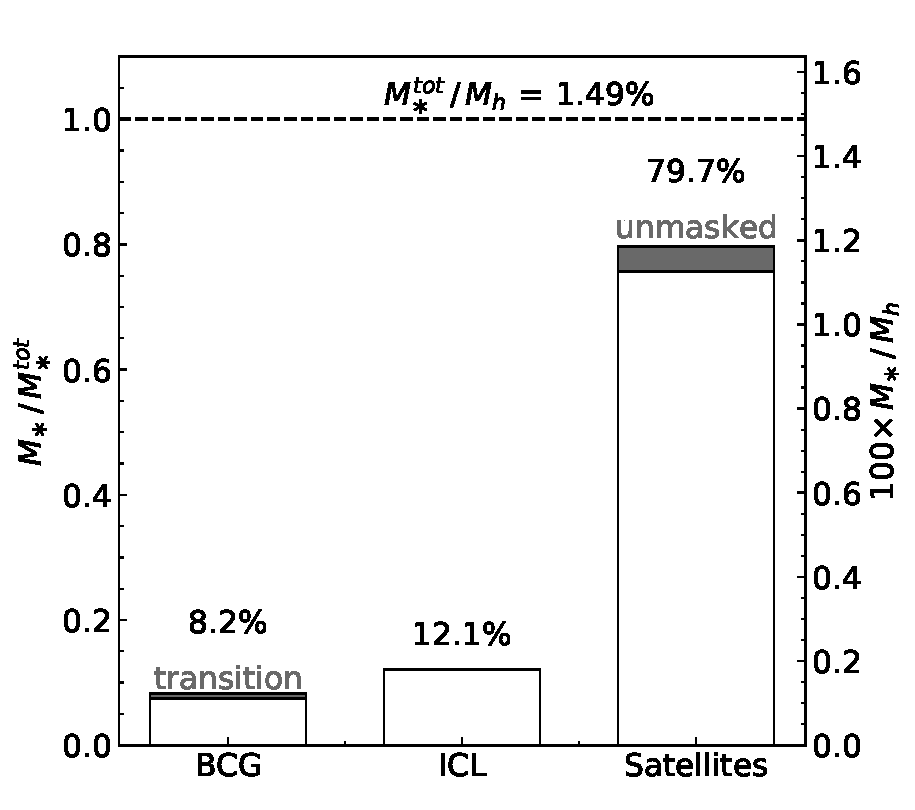
\includegraphics[width=0.48\textwidth]{fig/ICL_star_mass_fraction.pdf}
    \caption{Stellar mass budget of our cluster sample in BCG, ICl, and
    satellites. The gray shaded portions on top of the histograms for BCG
    and satellites represent the contributions from the transitional
    component and unmasked satellites, respectively. The stellar mass
    fraction and stellar-to-total mass ratio of each component are
    indicated by the left and right y-axes, respectively. The percentage
    value on top of each histogram indicates the stellar mass fraction of
    each component, while the horizontal line indicates the total
    stellar-to-halo mass fraction ratio of the clusters
    $M_*^{\mathrm{tot}}/M_h$.\label{fig:budget} }
\end{figure}


Finally, Figure~\ref{fig:budget} shows the stellar mass budget of our
cluster sample. We show the stellar mass fractions of the BCG, ICL, and
satellites in the left y-axis, and the stellar-to-halo mass fractions of
the three components in the right y-axis.  The ``transition'' portion
indicates the integrated mass within the $\sigtr$ profile~(\xkchen{$10^{10.57}\,\msol$})
shown in Figure~\ref{fig:decomposition}, while the ``unmasked'' portion
corresponds to the gray shaded region in Figure~\ref{fig:csmf}. The dashed
horizontal line in the top indicates the
total stellar mass-to-halo mass ratio~(\xkchen{$1.49\%$}) assuming a halo mass of \xkchen{$10^{14.49}\,\msol$}
measured from weak lensing in \citetalias{Zu2021}, significantly below the
cosmic baryon fraction of \xkchen{$15.74\%$ (under the adopted cosmology) }. Assuming further that the total baryon fraction of the clusters is the cosmic value \xkchen{$f_{b}=\Omega_{b} / \Omega_{m}$}~\citeme \xkchen{\citep{PlanckCollaboration2016} }, we can infer
that the \xkchen{$90.4\%$} of the baryons are in the form of the hot gas within
clusters.  For the stellar mass budget, \xkchen{$79.7\%$} of the stellar mass is
inside the satellite galaxies, while \xkchen{$8.2\%$} is in the BCG, leaving
\xkchen{$12.1\%$} of the stellar mass in the diffuse form of free-floating stars.

\ying{compare to the ICL numbers in the literature}
\xkchen{In observation, the ICL mass fraction in this work is consistent with the analysis of \citep{Morishita2017}. In \citep{Morishita2017}, they measured the ICL color and mass profiles of the six Hubble Frontier Field clusters with the deep \textit{Hubble Space Telescope (HST)} imaging data. Their result shows that the ICL stellar mass is $10^{11}$ to $10^{12}\,M_{\odot}$ and is about $5\%$ to $20\%$ of the total cluster stellar mass.}



\section{\texorpdfstring{$\rsoi$}{Rsoi}: Sphere of Influence of the BCG}
\label{sec:soi}

\begin{figure*}
    \centering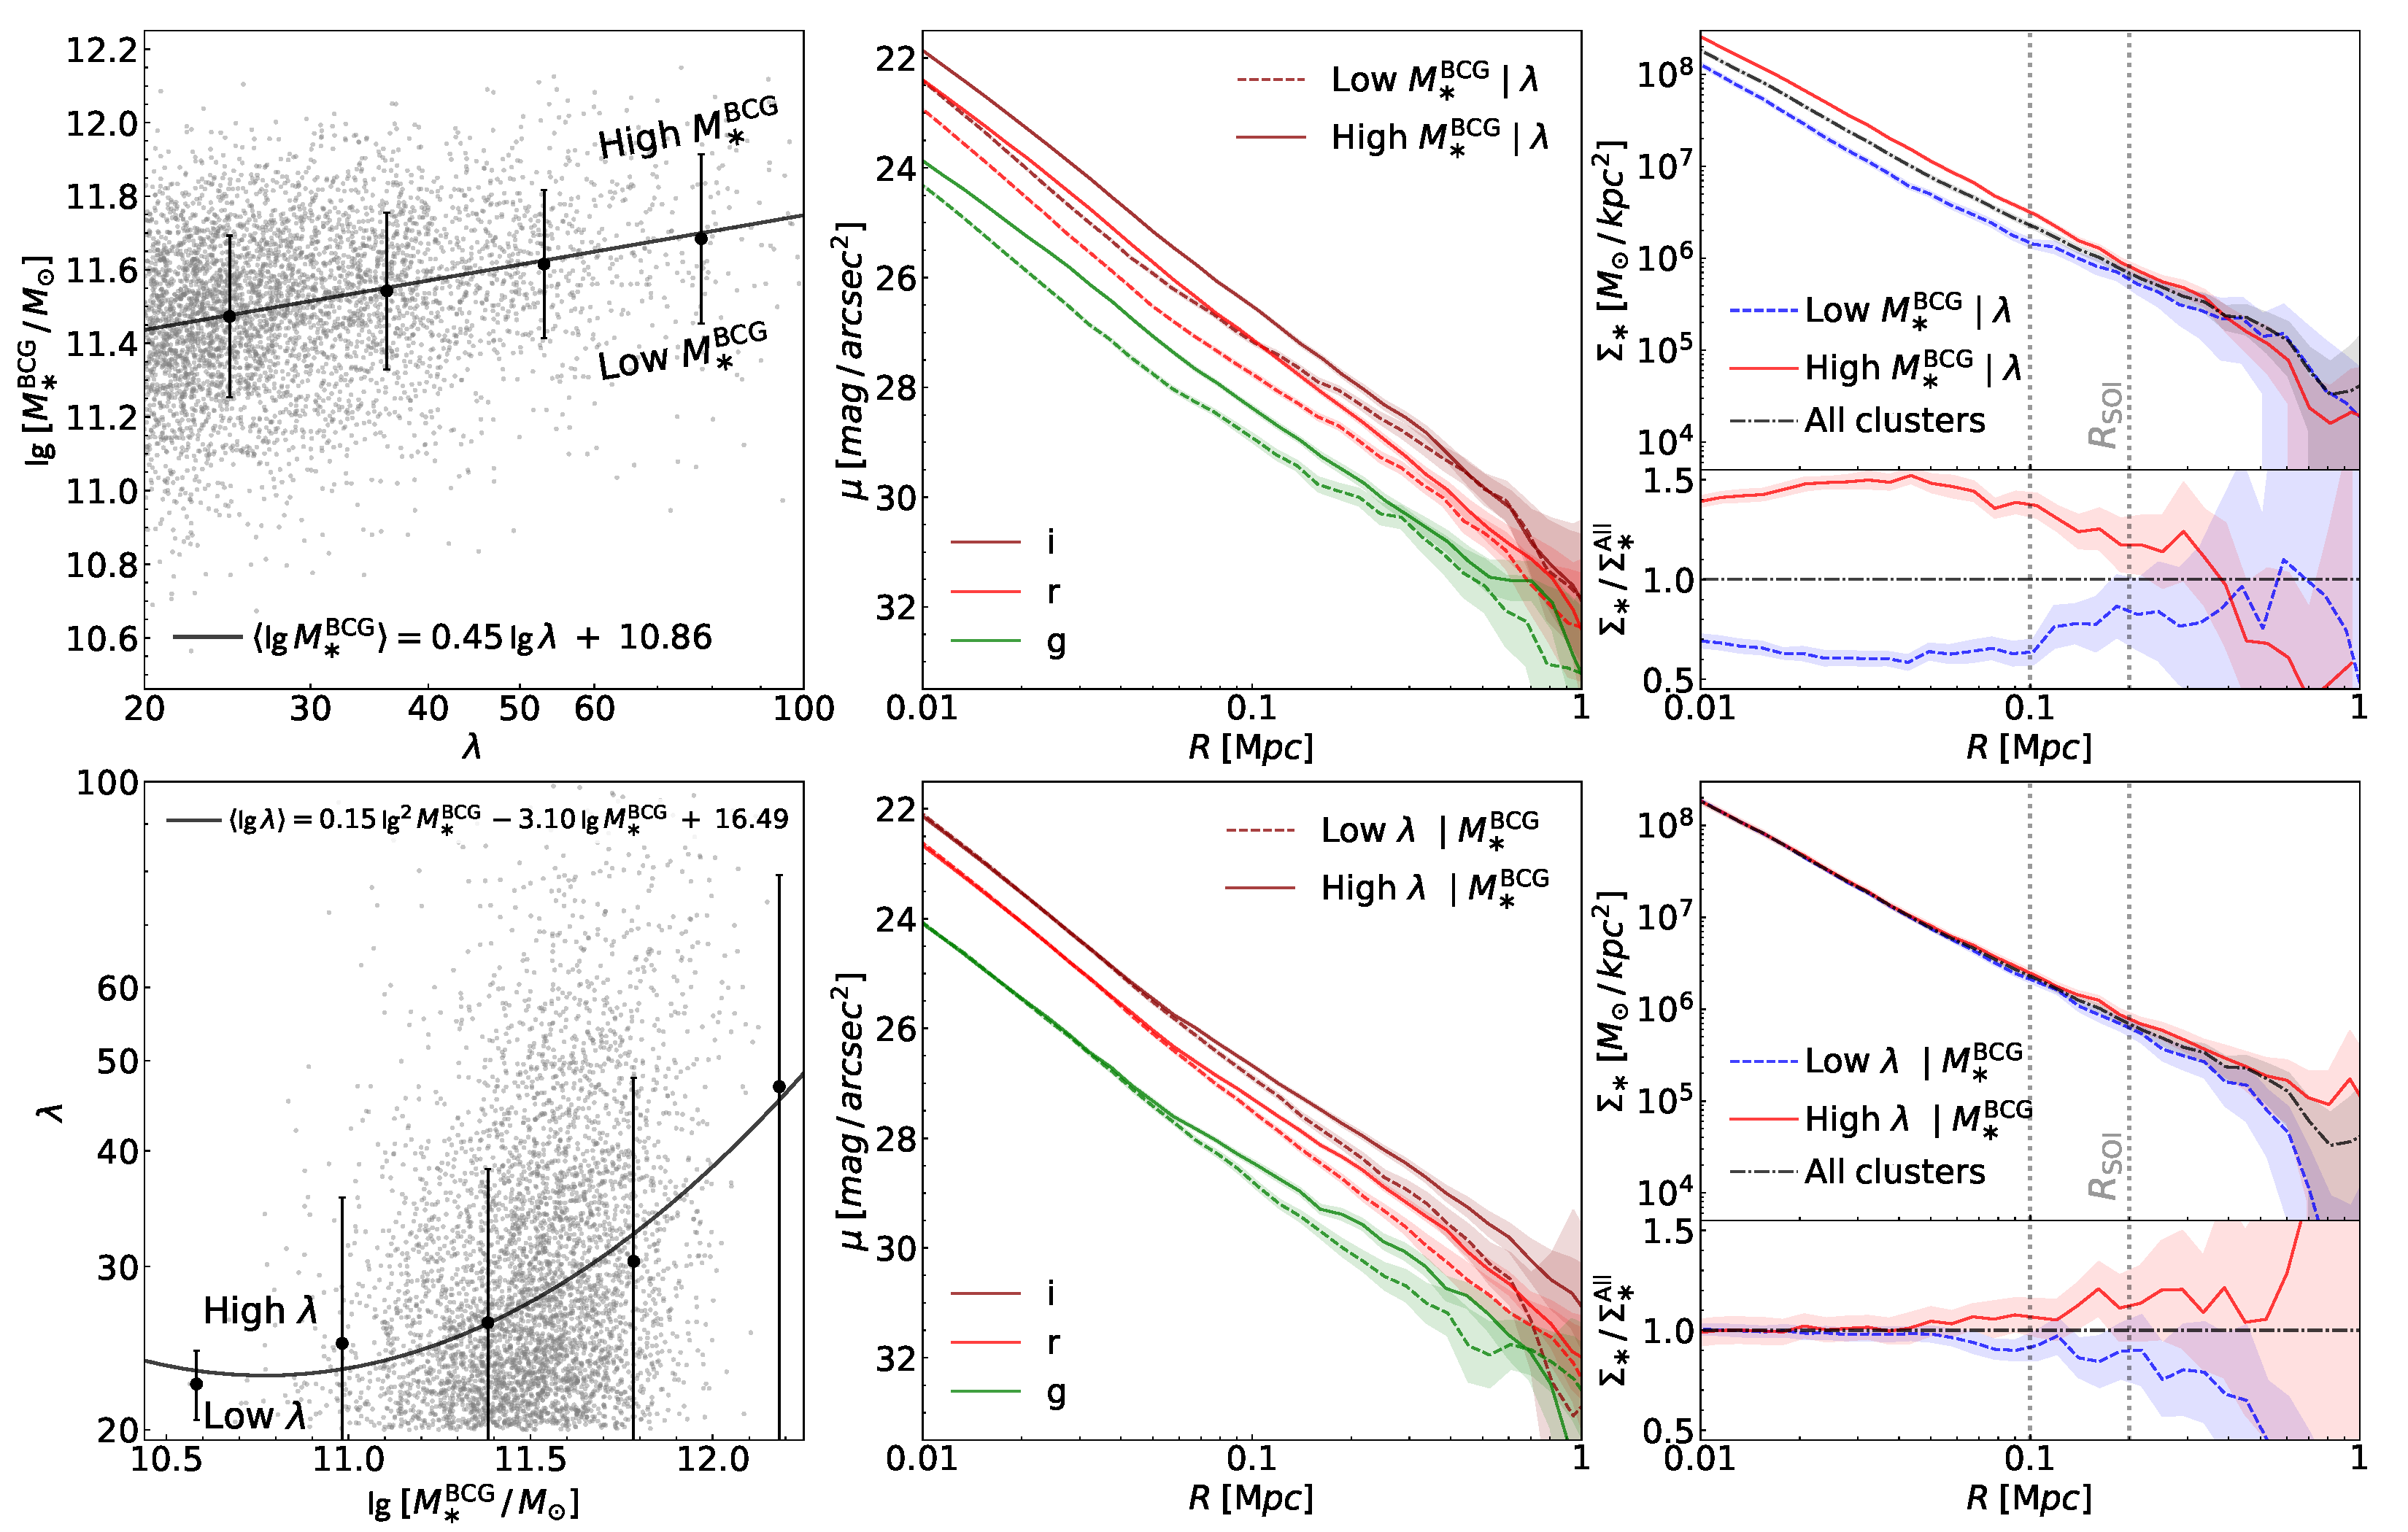
\includegraphics[width=0.96\textwidth]{fig/gri_subsample_result.pdf}
    \caption{Selection method~(left), surface brightness profiles~(middle),
    and stellar surface density profiles~(right) of cluster subsamples
    split by $\msbcg$~(top row) and $\lambda$~(bottom row).
	{\it Top left}: Distribution of clusters on the $\msbcg$ vs.
    $\lambda$ plane~(gray dots).  Black solid line is a linear fit to the
    median $\lg\msbcg$ at fixed $\lambda$, which divides the clusters into
    low and high-$\msbcg$ subsamples.  {\it Top middle}: Surface brightness
    profiles $\mubi$ of the low~(dashed curves) and high~(solid curves)
    $\msbcg$ subsamples. Green, red, and maroon curves indicate the
    measurements from $g$, $r$, and $i$-band images.  {\it Top right}:
    Stellar surface density profiles $\sigbi$ of the low-$\msbcg$~(blue
    dashed), high-$\msbcg$~(red solid), and all~(gray dot-dashed) clusters.
    The botttom subpanel shows the ratios of the $\sigbi$ profiles of the
    low~(blue dashed) and high~(red solid) $\msbcg$ subsamples over that of
    the overall sample. The panels in the bottom row are similar, but for
    the subsamples split by $\lambda$ at fixed $\msbcg$.\label{fig:split}}
\end{figure*}


Although we tentatively assign the transitional component to the BCG in
Figure~\ref{fig:budget}, it is unclear whether this stellar mass excess is
primarily induced by the BCG or the richness. Despite accounting
only for \xkchen{$4\%$} of the total stellar mass, this transitional component is
key to solving the sphere of influence of the BCGs $\rsoi$.  In particular,
if the excess mass is primarily richness-induced, we expect $\rsoi$ to stop
at ${\sim}50\kpc$; but a BCG-induced origin would extend $\rsoi$ beyond the
transitional component at ${\sim}200\kpc$. In this section, we divide our
overall cluster sample into two subsamples of different average BCG stellar
mass $\msbcg$, and aim to distinguish the two physical scenarios by
comparing the two sets of diffuse light and mass profiles.


\subsection{Cluster Subsamples Split by \texorpdfstring{$\msbcg$}{Mstar}}
\label{subsec:split}

\begin{figure*}
    \centering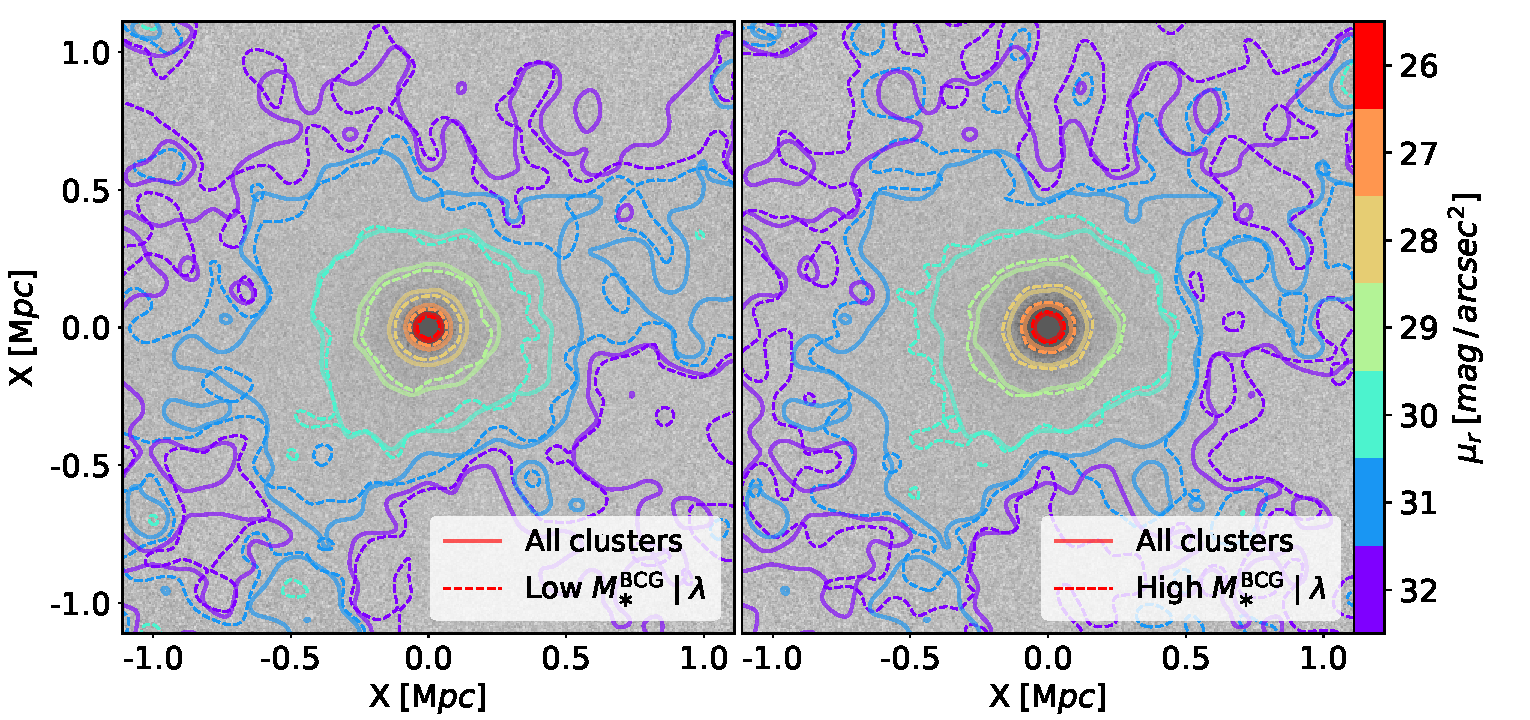
\includegraphics[width=0.96\textwidth]{fig/BCG_Mstar_bin_r-band_2D_signal.pdf}
    \caption{Comparison of the $r$-band stacked 2D image of the low~(left)
    and high~(right) $\msbcg$ subsamples. In each panel, dashed contour
    lines show the surface brightness distribution of the subsample, while
    the solid contours are for the overall sample, with the same
    colour-coding as in Figure~\ref{fig:2D_all} Below ${\sim}300\kpc$, the
    SB distribution of the low-$\msbcg$ subsample is generally fainter that
    that of the overall sample, which is then fainter than that of the
    high-$\msbcg$ subsample. On scales above ${\sim}500\kpc$, the three
    sets of contours are roughly consistent with one another.
    \label{fig:image2Dsub} }
\end{figure*}


Following \citetalias{Zu2021}, we split the clusters into two subsamples
using the median $\msbcg$-$\lambda$ relation, illustrated by the top left
panel in Figure~\ref{fig:split}. In particular, the median
$\msbcg$-$\lambda$ relation~(solid line) can be described by
\begin{equation}
    \xkchen{ \langle \lg M_{\ast}^{\mathrm{BCG}} \rangle = 0.45 \lg \lambda + 10.86 }
\end{equation}
dividing the clusters into two halves with the same distribution of
satellite richness $\lambda$, which we refer to simply as the
``high-$\msbcg$'' and ``low-$\msbcg$'' subsamples for the rest of the
paper. By applying the methods described in \S\ref{sec:sb} and
\S\ref{sec:sigma}, we measure the BCG+ICL surface brightness profile
$\mubi$~(top middle panel) and stellar surface mass profile $\sigbi$~(top
right panel) for each of the two subsamples.


In the top middle panel of Figure~\ref{fig:split}, solid and dashed curves
indicate the $\mubi(R)$ profiles of the high and low-$\msbcg$ subsamples,
respectively, in the SDSS $g$~(green), $r$~(red), and $i$~(maroon) bands.
By construction, the $\mubi(R)$ profile of the high-$\msbcg$ subsample is
\xkchen{$\sim0.56$} magnitudes brighter than that of the low-$\msbcg$ one on scales well
below the effective cModel aperture, i.e., $R_*{=}50\kpc$, because the
average $\msbcg$ of the two subsamples differ by \xkchen{$\sim0.28$} dex. However, the
small-scale discrepancy between the two subsamples persist on scales much
larger than $R_*$, and the two sets of $\mubi$ profiles do not converge
within the uncertainties until $R{\sim}300\kpc$. Likewise, the two $\sigbi$
profiles in the top right panel exhibit a significant discrepancy on scales
as large as $R{\sim}200{-}300\kpc$, beyond which they start to converge to
the same level of stellar surface mass density.


The comparison between the two $\sigbi$ profiles is better illustrated in
the bottom of the top right panel of Figure~\ref{fig:split}, where we show
the $\sigbi$ raitos of the low~(red solid) and high~(blue dashed) $\msbcg$
subsamples over the overall sample.  The discrepancy between the two raito
profiles is approximately a factor of two~(0.3 dex) across all scales below
$R{=}100\kpc$ before declining slowly on larger scales, but still persists
at ${\sim}30\%$ level at $R{\sim}200{-}300\kpc$.  Not until distances
exceed $R{\sim}300\kpc$ do the two ratio profiles begin to converge to
unity~(albeit with large errorbars).


Such discrepancy observed between the two subsamples provides a clear
detection of the BCG sphere of influence. Since the two subsamples of
clusters have the same richness and differ solely in their BCG stellar
mass, the clear transition from the constant discrepancy below
$R{=}100\kpc$ to the apparent convergence above $300\kpc$ in the top right
panel of Figure~\ref{fig:split} demonstrates that the BCG sphere of
influence extends to scales around $\rsoi{\sim}200\kpc$.
Interestingly, such transition at $\rsoi$ coincides with the radial extent
of the transitional stellar mass component revealed by the $\sigbi$
decomposition in \S\ref{subsec:decomposition}, suggesting a common origin
of the two observed ``transitions''. In particular, the excess diffuse
light on scales between $R_*$ and $\rsoi$ should be primarily formed via
processes that simultaneously enriched the BCG, likely due to the tidal
disruption/stripping of satellites after periapsis and the stellar ejection
from mergers between the BCGs and satellites. Furthermore, the convergence
of the two $\sigbi$ profiles on scales above $300\kpc$ confirms our
expectation that the ICL in the outer region of clusters largely follows
the distribution of satellite galaxies, hence that of the dark matter.


The bottom panels of Figure~\ref{fig:split} shows the results of a similar
experiment as in the top panels, but by dividing the clusters into low and
high-$\lambda$ subsamples by the richness $\lambda$ at fixed BCG stellar
mass $\msbcg$~(bottom left panel). As expected, the two sets of $\mubi$ and
$\sigbi$ profiles are consistent on scales below $R_*{=}50\kpc$, but start
to differ on scales above, reaching
a discrepancy of $20\%$ at $R{\sim}200\kpc$. Overall, the discrepancy
between the low and high-$\lambda$ clusters is significantly smaller than
that between the two $\msbcg$-split halves on scales between $50\kpc$ and
$200\kpc$, indicating that the influence of satellite richness is
subdominant compared to the BCG on those transitional scales --- they are
firmly within the sphere of influence of the BCG.



Figure~\ref{fig:image2Dsub} provides a more visually-apealing way of
comparing the diffuse light distributions between the low and high-$\msbcg$
subsamples.  In particular, we compare the 2D stacked $r$-band images of
the low-$\msbcg$~(left) and high-$\msbcg$~(right) subsamples~(dashed
contours) to that of the overall sample~(solid contours in both panels;
same as in Figure~\ref{fig:2D_all}). Consistent with 1D profiles in the top
panels of Figure~\ref{fig:split}, the high-$\msbcg$ clusters exhibits a
more enhanced surface brightness distribution than the low-$msbcg$ systems
on scales below $300\kpc$, but the two images are almost indistinguishable
on scales above $500\kpc$.


\subsection{Systematic Tests Against Stellar Mass Aperture and BCG
Centering Probability}
\label{subsec:test}


The key conclusion of our paper, that the BCG sphere of influence extends
to a characteristic radius of $\rsoi{\simeq}200\,\kpc$, is based on the
experiments of \S~\ref{subsec:split}. However, the experiments could be
affected by systematic uncertainties associated with the aperture of our
stellar mass estimates or the miscentring effect in the \redmapper~cluster
finding algorithm~\citeme \xkchen{\citep{Johnston2007, Oguri2011, Rozo2014, Hollowood2019} }. For example, although the effective aperture of
$\msbcg$ is $R_*{\sim}50\kpc$, the individual apertures of some of the
nearby, bright systems could be larger, thereby artificially pushing the
discrepancy between the $\sigbi$ of high and low-$\msbcg$ subsample to
larger radii. For miscentring, the average centring probability $\pcen$ of
the low-$\msbcg$ clusters is lower, and is thus more likely to have
satellite galaxies misidentified as centrals than their high-$\msbcg$
counterparts. Consequently, it is plausible that the $\sigbi$ of the
low-$\msbcg$ subsample is heavily underestimated on small scales due to the
lack of extended stellar envelope surrounding those misidentified centrals.



To investigate the impact of different apertures, we repeat the experiment
of \S~\ref{subsec:split} by adopting $\mtwenty$, the stellar mass measured
within a fixed aperture of $20\kpc$. By splitting the clusters into two
subsamples of different $\mtwenty$ at fixed $\lambda$, we eliminate the
possibility that the high-$msbcg$ subsample may preferentially select the
larger BCGs. The result of this test is shown as the red~(high-$\mtwenty$)
and blue~(low-$\mtwenty$) dashed curves in Figure~\ref{fig:systest}.  The
$\sigbi$ of the high-$\mtwenty$ subsample is \xkchen{$\sim2.6$} per cent lower than that
of the high-$\msbcg$ clusters on scales below $200\kpc$, while the $\sigbi$
of the low-$\mtwenty$ subsample is largely consistent with that of the
low-$\msbcg$ clusters on all scales.\xkchen{while the $\sigbi$ of the low-$\mtwenty$ subsample is $\sim2.1$ per cent higher than that of the low-$\msbcg$ subsample.} Overall, the discrepancy between the
$\sigbi$ profiles of the two subsamples split by $\mtwenty$ is very similar
to our fiducial measurement split by $\msbcg$~(solid curves), consistent
with the BCG sphere of influence extending to $\rsoi{\sim}200\kpc$.



To test the miscentring effect, we measure the $\pcen$ distributions of the
BCGs of the high~(red histograms) and low~(blue histograms) $\msbcg$
subsamples in the inset panel of Figure~\ref{fig:systest}.  Both $\pcen$
distributions peak close to 100\%, but the distribution of the low-$\msbcg$
clusters indeed exhibits a longer low-$\pcen$ tail. To eliminate the impact
of low-$\pcen$ systems on our $\rsoi$ measurement, we remove clusters with
the $\pcen$ of their BCGs lower than 85\%, shown as the vertical dashed
line in the inset panel, and redo the analysis using the $\msbcg$-split
subsamples.  The results of the miscentring test are shown by the red and
blue dotted curves for the high and low-$\msbcg$ clusters with BCG
$\pcen{>}85\%$, respectively. Again, we do not find any significant
deviation from our fiducial measurements due to
the exclusion of the low-$\pcen$ systems.


Therefore, based on the two systematic tests shown in
Figure~\ref{fig:systest}, we conclude that the detection of
$\rsoi{\sim}200\kpc$ is robust against the aperture size of the BCG
stellar mass estimates and the level of miscentring in the SDSS
\redmapper~catalogue.




\subsection{Connection between BCG Sphere of Influence and Halo Concentration}
\label{subsec:physics}


\begin{figure}
    \hspace{-0.5cm}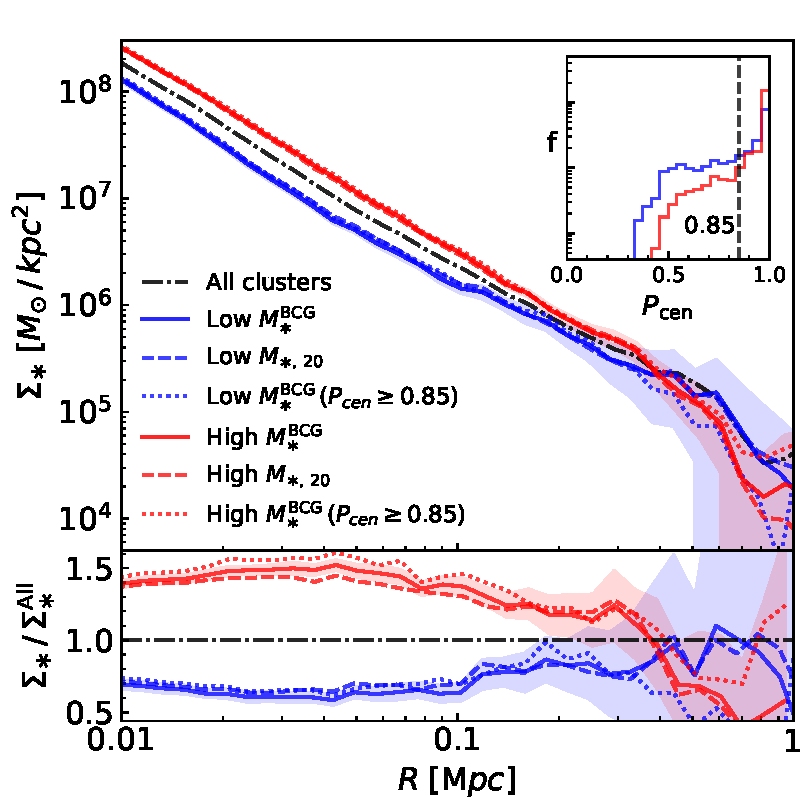
\includegraphics[width=0.48\textwidth]{fig/M-bin_SM_compare.pdf}
    \caption{Similar to the top right panel of Figure~\ref{fig:split}, but
    with measurements for cluster subsamples split by $\mtwenty$~(stellar
    mass measured within a $20\kpc$ aperture; dashed curves) and for
    clusters with BCG centring probability $\pcen{>}0.85$~(dotted curves).
    Inset panel shows the $\pcen$ distributions of the low~(blue
    histograms) and high~(red histograms) $\msbcg$ subsamples, with the
    vertical dashed line indicating our $\pcen{=}0.85$ cut.
    \label{fig:systest} }
\end{figure}


As mentioned in the Introduction, \citetalias{Zu2021} modelled the weak
lensing measurements of the two subsamples split by $\msbcg$ at fixed
$\lambda$, and found that the two have the same average halo mass, but the
average halo concentration of the high-$\msbcg$ clusters is
${\sim}10\%$ higher than that of the low-$\msbcg$ systems~(for a thorough
explanation of such observation, see Zu et al. 2021b~\citeme \xkchen{\citep{Zu2021b} } \xkchen{Zu et al. 2021a cannot change after compiling}).
\citetalias{Zu2021} speculated that the strong correlation between halo
concentration and $\msbcg$ could be induced at the early phase of halo
growth, when the fast accretion and frequent mergers not only built the
characteristic cores of the cluster haloes, but also fuel the {\it in situ}
stellar growth of the BCGs. Interestingly, the characteristic radii $r_s$
inferred by \citetalias{Zu2021} are ${\sim}200{-}300\kpc$, in good
agreement with our constraint of $\rsoi$ in this paper.


\begin{figure*}
    \centering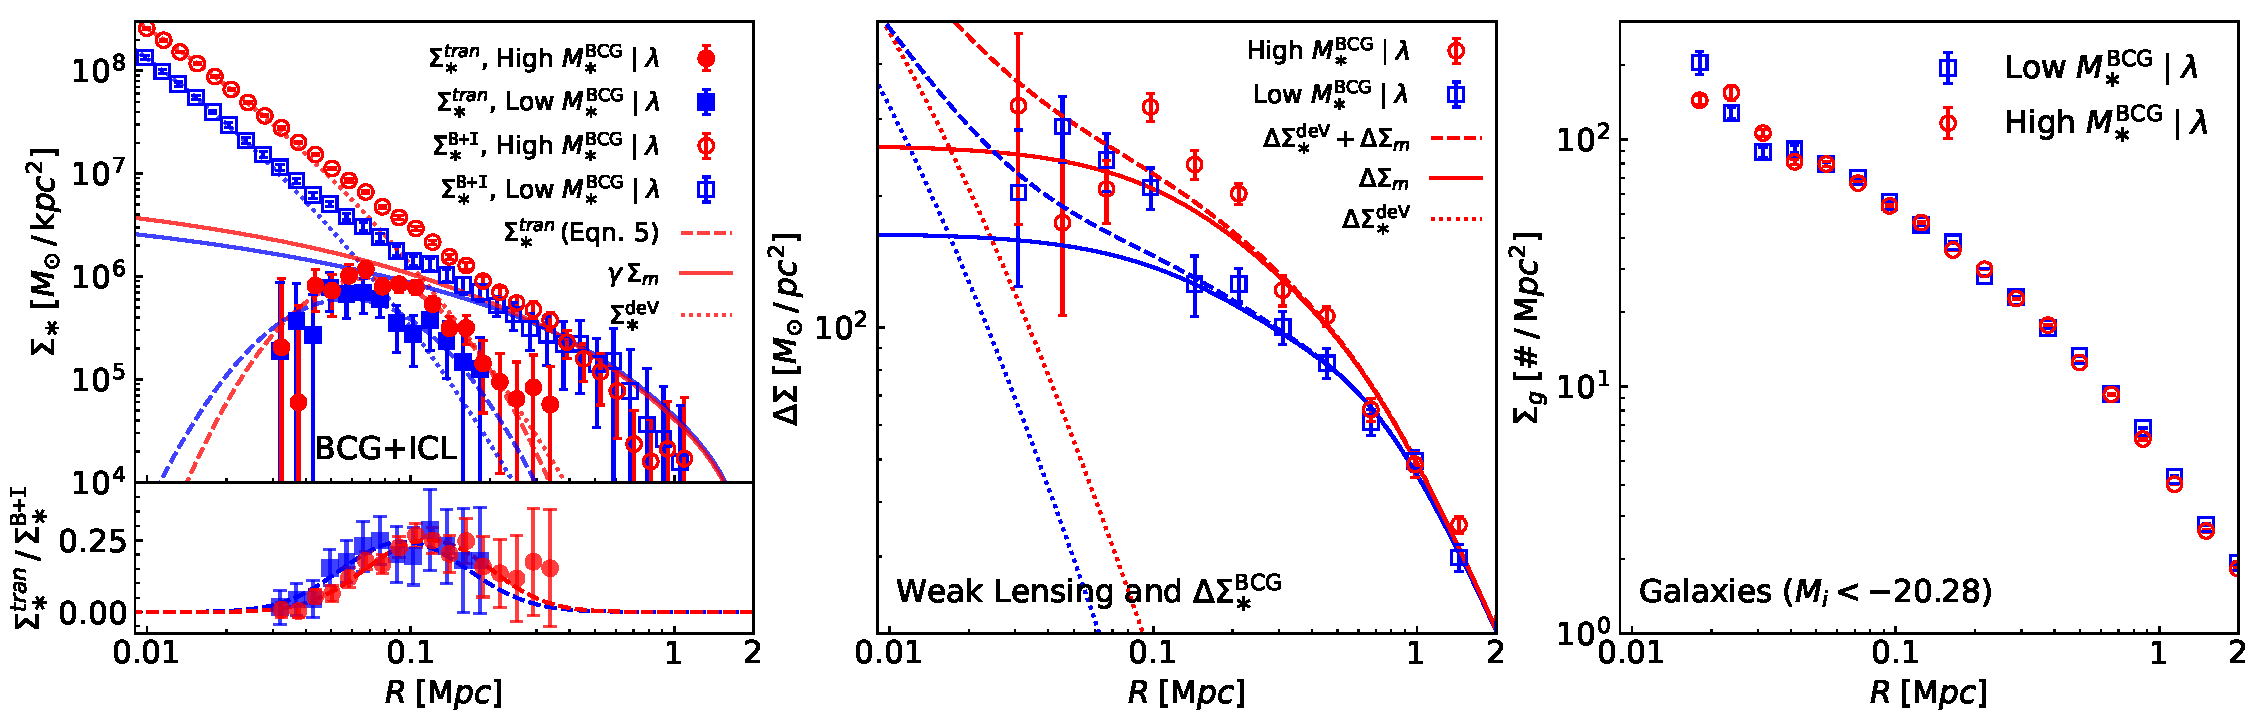
\includegraphics[width=0.96\textwidth]{fig/subsamples_SB_SM.pdf}
    \caption{{\it Left}: BCG+ICL stellar surface density profiles $\sigbi$
    of the low~(blue open squares) and high (red open circles) $\msbcg$
    subsamples. Solid and dotted curves are the best-fitting scaled matter
    density and de Vaucouleurs' profiles on relevant scales, respectively.
    Blue filled squares and red filled circles indicate the transitional
    components of the low and high-$\msbcg$ clusters, respectively, while
    the dashed curves are the best-fitting log-normal functions.  {\it
    Middle}: Weak lensing profiles $\ds$ of the low~(blue open squares) and
    high (red open circles) $\msbcg$ subsamples. Solid curves are the
    predictions by the best-fitting $\ds$ models described in
    \citetalias{Zu2021}. The two $\ds$ models have the same halo mass, but
    the average halo concentration of the high-$\msbcg$ subsample is
    ${\sim}10\%$ higher than that of the low-$\msbcg$ clusters. Dotted
    curves indicate the predicted $\ds$ signal induced by the respective de
    Vaucouleurs' profiles shown in the left panel, and each dashed curve is
    the sum of the dotted and solid curves of the same colour.  {\it
    Right}: The galaxy surface number density profiles $\sigg$ of the
    low~(blue open squares) and high (red open circles) $\msbcg$
    subsamples. The two measured profiles are consistent with each other on
all scales. \label{fig:subdecomposition}}
\end{figure*}


Such similarity between the values of $r_s$ and $\rsoi$ is likely physical.
In the vicinity of the BCGs, stars could be tidally disrupted/stripped from
satellites after periapsis or ejected from BCG-satellite mergers. Most of
those stray stars cannot escape to larger radii due to the relatively high
escape velocities within $r_s$. Therefore, a fraction of them would fall
back onto the BCGs and grow $\msbcg$, while the rest stays unbound to the
BCGs and form the transitional component $\sigtr$, which is however well
confined within the BCG sphere of influence $\rsoi$. In this scenario, the
BCG sphere of influence is partly maintained by the central core of the
halo. Future observations with even larger cluster samples and deeper
photometry could potentially clarify the existence of this $r_s$-$\rsoi$
connection.


Finally, we present a comprehensive comparison between the low~(blue
squares) and high~(red circles) $\msbcg$ subsamples in their BCG+ICL
stellar surface density profiles $\sigbi$~(left), weak lensing profiles
$\ds$~(middle), and galaxy surface number density profile $\sigg$~(right)
in Figure~\ref{fig:subdecomposition}. The left panel is similar to
Figure~\ref{fig:decomposition}, but with our decomposition method applied
to the two subsamples separately.  The integrated mass within the
transitional component $\sigtr$ of the high-$\msbcg$ subsample~(red filled
circles) is \xkchen{$10^{10.82}\msol$} , \xkchen{${\sim}0.27$} dex higher than that of the low-$\msbcg$
subsample~(blue filled squares), \ying{consistent?larger?smaller?}\xkchen{smaller} with the
\xkchen{$0.28$} dex discrepancy between the two average $\msbcg$.



The middle panel of Figure~\ref{fig:subdecomposition} is similar to the
Figure 5 of \citetalias{Zu2021}, showing the weak lensing comparison
between the two subsamples. We also include the weak lensing signals
predicted on small scales by the de Vaucouleurs' profiles of the
BCGs~(dotted curves) in the prediction of the total
$\ds$~(dashed curves). The $10\%$ difference in halo concentration is
manifested by the large discrepancy between the two $\ds$ profiles on
scales between $100\kpc$ and $500\kpc$. We show the comparison between the
two galaxy surface number density profiles in the right panels of
Figure~\ref{fig:subdecomposition}~(similar to the right panel of Figure 6
in \citetalias{Zu2021}). Clearly, the galaxy distributions around the BCGs
of the two subsamples are almost indistinguishable, indicating that the
differences in $\sigbi$~(left) and $\ds$~(middle) are tied solely to the
discrepancy in $\msbcg$. The remarkable similarity between the two $\sigg$
profiles also confirms our expectation that the richness-induced ICL
profiles between the two subsamples should be the same.


\section{Conclusion}
\label{sec:conc}

\section*{Data availability}

The data underlying this article will be shared on reasonable request to the corresponding author.


\section*{Acknowledgements}

We thank \xxx for helpful
discussions.  XKC and YZ acknowledge the support by the National Key Basic
Research and Development Program of China (No.  2018YFA0404504), National
Science Foundation of China (11873038, 11621303, 11890692), and the science
research grants from the China Manned Space Project (No.
CMS-CSST-2021-A01, CMS-CSST-2021-B01). YZ acknowledges the National
One-Thousand Youth Talent Program of China, the SJTU start-up fund (No.
WF220407220), and the support by the 111 Project of the Ministry of
Education under grant No. B20019. YZ thanks the wonderful hospitality by
Cathy Huang during his visit at the Zhangjiang Hi-Tech Park during the
summer of 2021.



%%%%%%%%%%%%%%%%%%%% REFERENCES %%%%%%%%%%%%%%%%%%

% The best way to enter references is to use BibTeX:

% \clearpage
\bibliographystyle{mnras}
%\bibliography{ref} %
\bibliography{ref_me.bib}

% Alternatively you could enter them by hand, like this:
% This method is tedious and prone to error if you have lots of references
% \begin{thebibliography}{99}
% \bibitem[\protect\citeauthoryear{Author}{2012}]{Author2012}
% Author A.~N., 2013, Journal of Improbable Astronomy, 1, 1
% \bibitem[\protect\citeauthoryear{Others}{2013}]{Others2013}
% Others S., 2012, Journal of Interesting Stuff, 17, 198
% \end{thebibliography}
\begin{thebibliography}{}
\makeatletter
\relax
\def\mn@urlcharsother{\let\do\@makeother \do\$\do\&\do\#\do\^\do\_\do\%\do\~}
\def\mn@doi{\begingroup\mn@urlcharsother \@ifnextchar [ {\mn@doi@}
  {\mn@doi@[]}}
\def\mn@doi@[#1]#2{\def\@tempa{#1}\ifx\@tempa\@empty \href
  {http://dx.doi.org/#2} {doi:#2}\else \href {http://dx.doi.org/#2} {#1}\fi
  \endgroup}
\def\mn@eprint#1#2{\mn@eprint@#1:#2::\@nil}
\def\mn@eprint@arXiv#1{\href {http://arxiv.org/abs/#1} {{\tt arXiv:#1}}}
\def\mn@eprint@dblp#1{\href {http://dblp.uni-trier.de/rec/bibtex/#1.xml}
  {dblp:#1}}
\def\mn@eprint@#1:#2:#3:#4\@nil{\def\@tempa {#1}\def\@tempb {#2}\def\@tempc
  {#3}\ifx \@tempc \@empty \let \@tempc \@tempb \let \@tempb \@tempa \fi \ifx
  \@tempb \@empty \def\@tempb {arXiv}\fi \@ifundefined
  {mn@eprint@\@tempb}{\@tempb:\@tempc}{\expandafter \expandafter \csname
  mn@eprint@\@tempb\endcsname \expandafter{\@tempc}}}


\makeatother
\end{thebibliography}


%%%%%%%%%%%%%%%%%%%%%%%%%%%%%%%%%%%%%%%%%%%%%%%%%%

% Don't change these lines
\bsp	% typesetting comment
\label{lastpage}

\end{document}
